\documentclass{beamer}
\usetheme[faculty=med]{fibeamer}
\usepackage[utf8]{inputenc}
\usepackage[
  main=english
]{babel}        %% typeset as follows:
%% These macros specify information about the presentation
\title{Sistemas Operacionais} %% that will be typeset on the
\subtitle{Introdução} %% title page.
\author{Guilherme Meira}
%% These additional packages are used within the document:
\usepackage{ragged2e}  % `\justifying` text
\usepackage{booktabs}  % Tables
\usepackage{tabularx}
\usepackage{tikz}      % Diagrams
\usetikzlibrary{calc, shapes, backgrounds, positioning}
\usepackage{minted}
\usepackage{amsmath, amssymb}
\usepackage{url}       % `\url`s
\usepackage{listings}  % Code listings
\usepackage{xcolor}
\definecolor{highlightcolor}{RGB}{255, 140, 119}
\setminted{highlightcolor=highlightcolor}
\frenchspacing
\begin{document}
  \frame{\maketitle}
  \AtBeginSection[]{% Print an outline at the beginning of sections
  	\begin{frame}<beamer>
  		\frametitle{Agenda}
  		\tableofcontents[currentsection]
  	\end{frame}}
  	
\section{Apresentação da disciplina}
\begin{frame}{Apresentação da disciplina}
   	\begin{itemize}
   		\item[Disciplina] Sistemas Operacionais
   		\item[Professor] Guilherme Meira
   		\item[Horário] Quartas-feiras, das 18:50h às 22:00h
   		\begin{itemize}
   			\item Intervalo de 10 minutos por volta das 20:20h
   			\item Chamada ao final da aula
   		\end{itemize}
   		\item[Avaliação] Duas provas + duas avaliações multidisciplinares
   		\begin{itemize}
   			\item 7 pontos de prova ($P_{1}$ e $P_{2}$)
   			\item 3 pontos de Avaliação Multidisciplinar ($T_{1}$ e $T_{2}$)
   			\item $M_{P} = \frac{P_{1} + T_{1} + P_{2} + T_{2}}{2}$
   			\item $M_{P} \ge 7$: aprovado
   			\item $M_{P} < 7$: prova final ($P_{F}$)
   			\item $M_{F} = \frac{M_{P} + P_{F}}{2}$
   			\item $M_{F} \ge 5$: aprovado
   			\item $M_{F} < 5$: gostou  tanto da matéria que vai fazer de novo
   		\end{itemize}
   	\end{itemize}
\end{frame}
\begin{frame}{Apresentação da disciplina}
   	\begin{itemize}
   		\item[Trabalhos] Avaliação Multidisciplinar
   		\begin{itemize}
   			\item Individual
   			\item Questões objetivas
   		\end{itemize}
   		\item[Livro] Sistemas Operacionais Modernos (Andrew S. Tanenbaum)
   		\item[Outros]
   		\begin{itemize}
   			\item Honestidade acadêmica
   			\item Comportamento em sala
   			\item Feedback!
   		\end{itemize}
   	\end{itemize}
\end{frame}

\section{Introdução}
\begin{frame}{Introdução}
	\textbf{Tarefa:} Escreva um programa que multiplique um número por 2 e mostre o resultado.
	\pause
	\inputminted{c}{resources/helloworld.c}
	\pause
	Agora faça o mesmo sem usar um sistema operacional.
	\begin{tikzpicture}[overlay, remember picture]
	\node[anchor=south east, yshift=20, xshift=-20] at (current page.south east) {
		
\includegraphics[width=0.15\paperwidth]{resources/troll}
	};
	\end{tikzpicture}
\end{frame}
\begin{frame}{Introdução}
	\textbf{Passo 1:} Ler o programa do disco
	\begin{figure}
		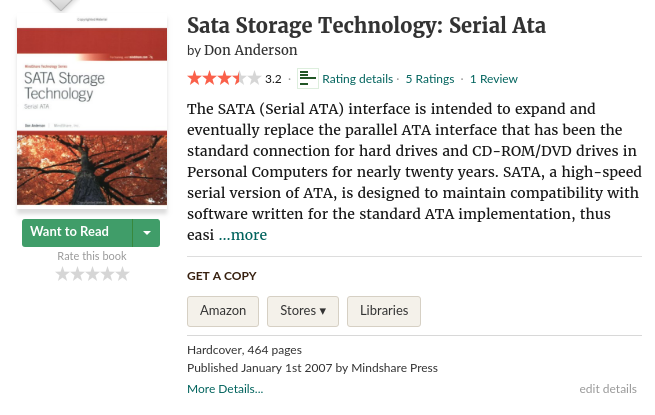
\includegraphics[width=0.7\paperwidth]{resources/sata}
	\end{figure}
\end{frame}
\begin{frame}{Introdução}
	\textbf{Passo 2:} Carregar o programa na memória
	\begin{figure}
		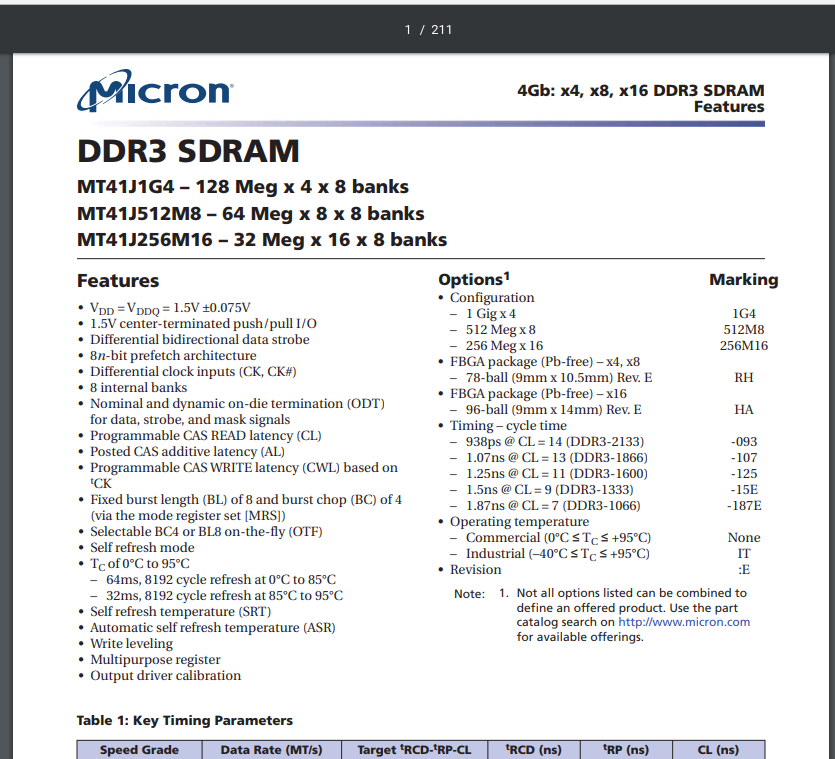
\includegraphics[width=0.6\paperwidth]{resources/ram}
	\end{figure}
\end{frame}
\begin{frame}{Introdução}
	\textbf{Passo 2:} Carregar o programa na memória
	\begin{figure}
		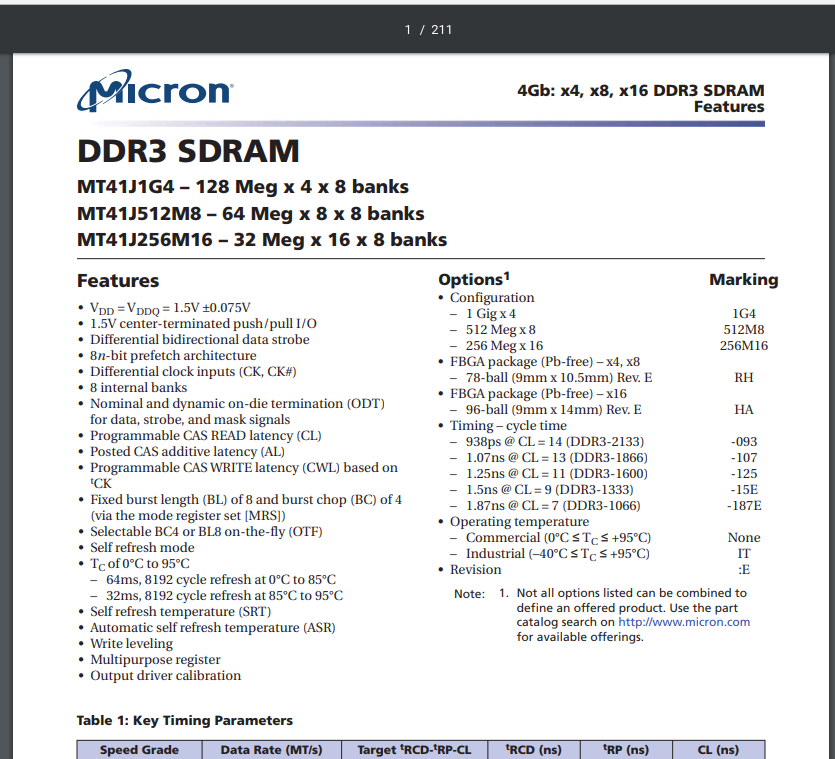
\includegraphics[width=0.6\paperwidth]{resources/ram}
	\end{figure}
\end{frame}
\begin{frame}{Introdução}
	\textbf{Passo 3:} Exibir algo na tela
	\begin{figure}
		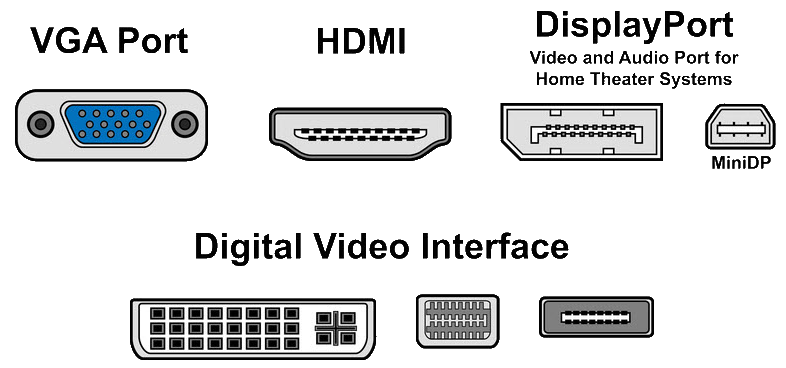
\includegraphics[width=0.6\paperwidth]{resources/video}
	\end{figure}
\end{frame}
\begin{frame}{Introdução}
	\textbf{Passo 4:} Obter entrada pelo teclado
	\begin{figure}
		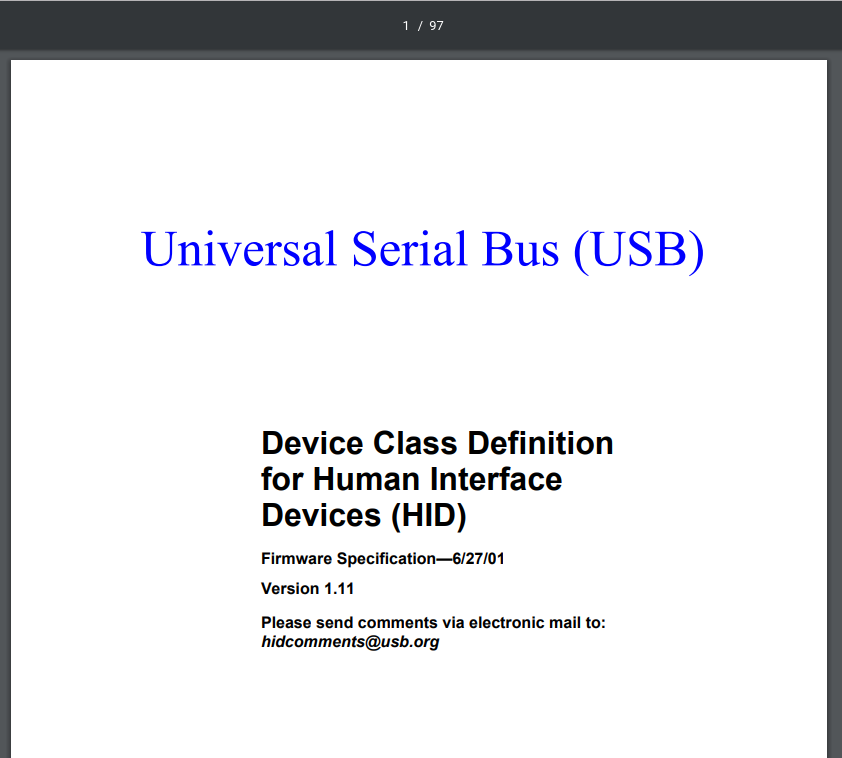
\includegraphics[width=0.6\paperwidth]{resources/usb}
	\end{figure}
\end{frame}
\begin{frame}{Introdução}
	\begin{itemize}
		\item E se precisar se comunicar via rede?
		\item E se vários processos precisarem executar ao mesmo tempo?
		\item Mouse?
		\item Interface gráfica?
		\item Audio?
	\end{itemize}
	\pause
	\begin{figure}
		
\includegraphics[width=0.4\paperwidth]{resources/please}
	\end{figure}
\end{frame}
\begin{frame}{Introdução}
	\textit{``Sistemas Operacionais transformam a feiura do hardware em interfaces bonitas.''}
	\begin{figure}
		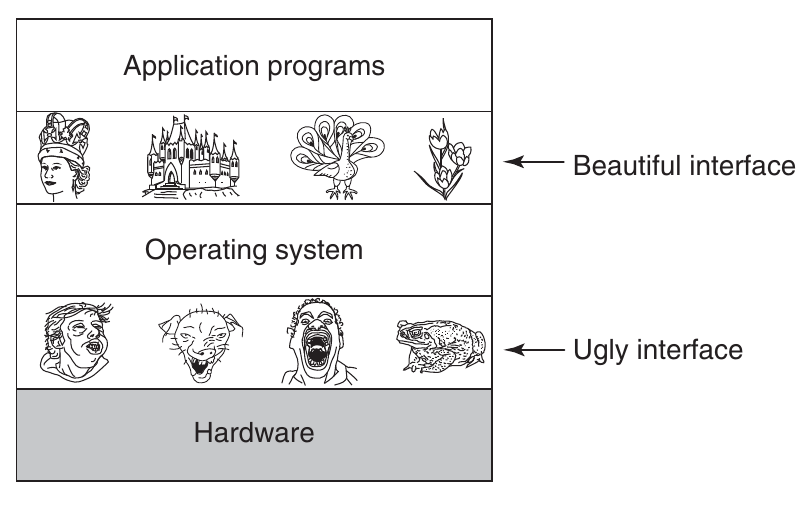
\includegraphics[width=0.6\paperwidth]{resources/ugly}
	\end{figure}
\end{frame}

\section{Histórico}
\begin{frame}{Histórico}
	\framesubtitle{Século 19}
	\begin{itemize}
		\item Charles Babbage
		\item Primeiro computador digital - ``Máquina Analítica''
		\item Puramente mecânico
		\item Tecnologia da época não era suficiente
		\item Primeira programadora: Ada Lovelace
	\end{itemize}
	\begin{tikzpicture}[overlay, remember picture]
	\node[anchor=north east, yshift=-20, xshift=-20] at (current page.north east) {
		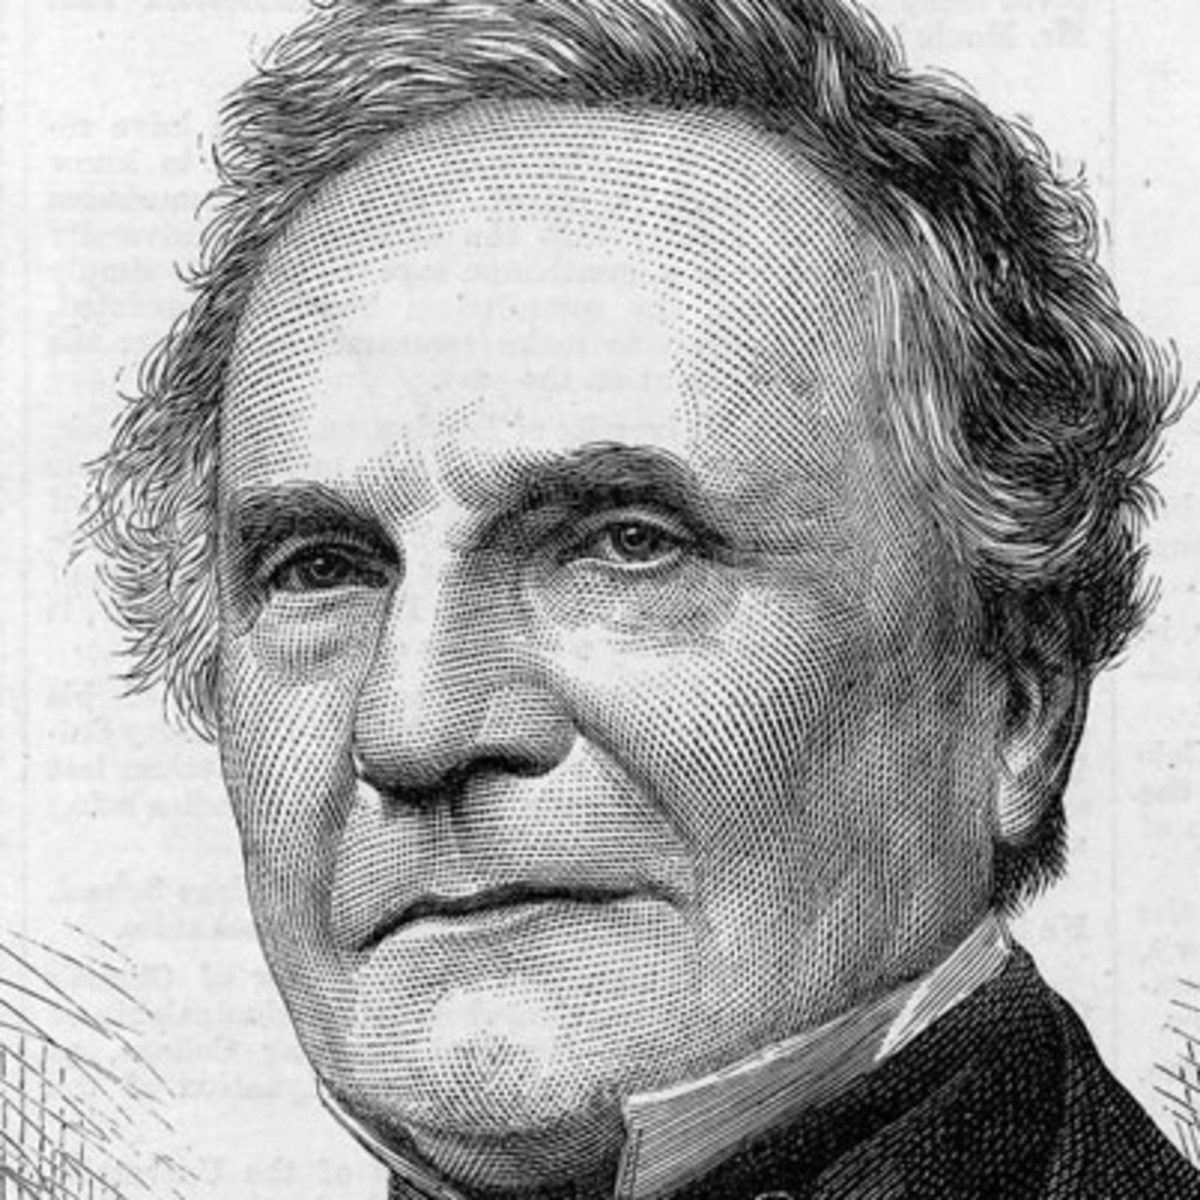
\includegraphics[width=0.2\paperwidth]{resources/babbage}
	};
	\node[anchor=south east, yshift=20, xshift=-20] at (current page.south east) {
		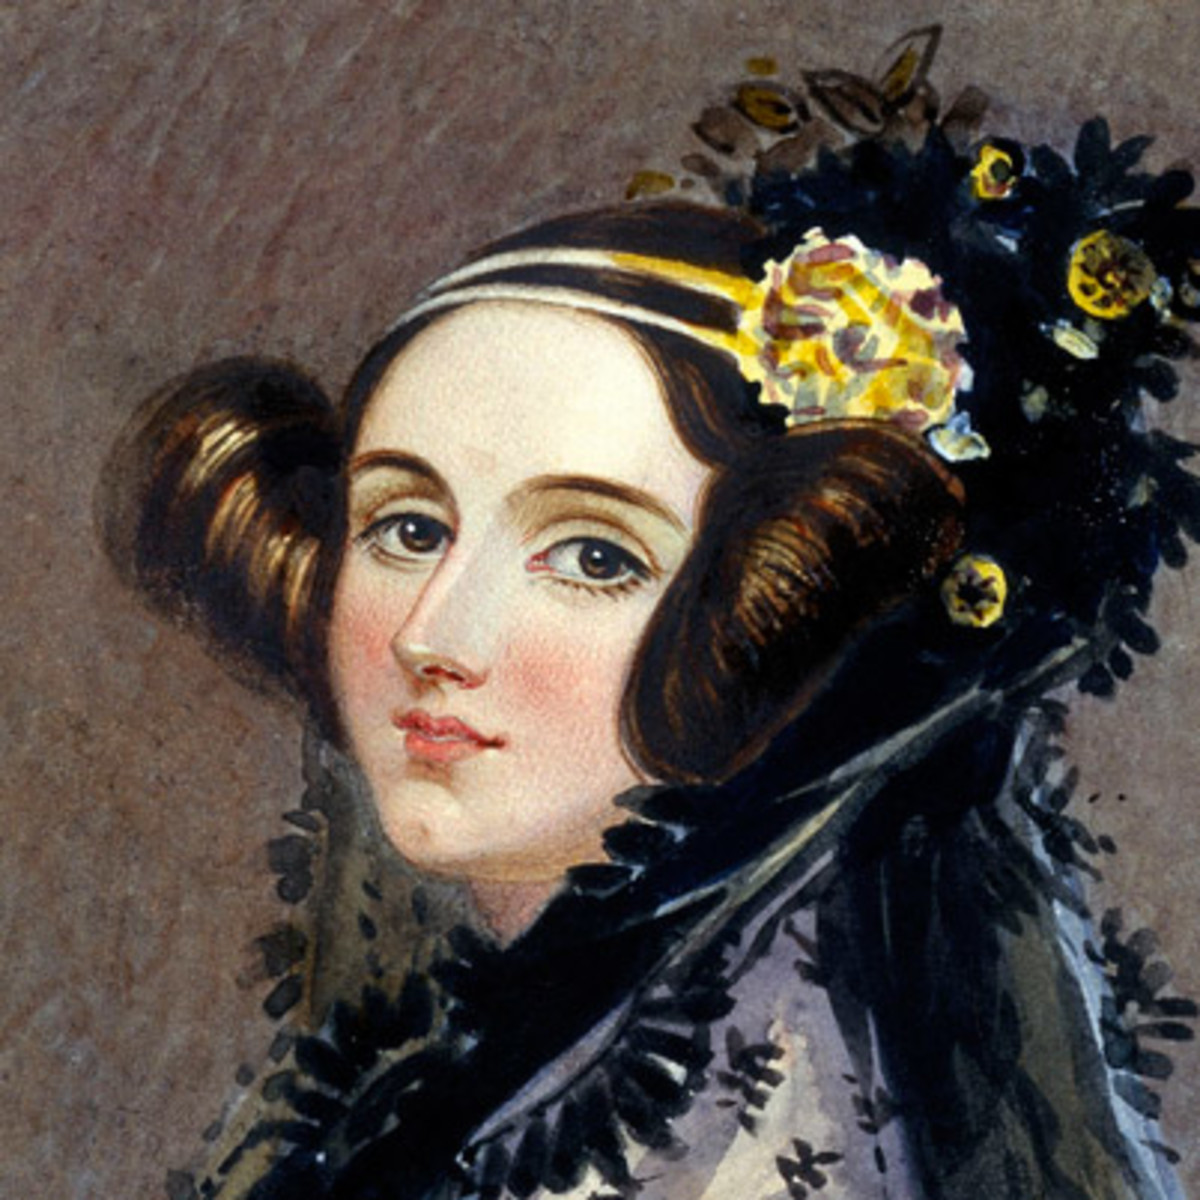
\includegraphics[width=0.2\paperwidth]{resources/ada}
	};
	\node[anchor=south west, yshift=10, xshift=20] at (current page.south west) {
		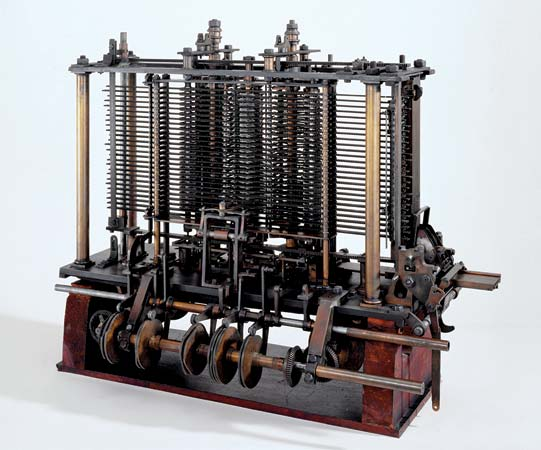
\includegraphics[width=0.2\paperwidth]{resources/engine}
	};
	\end{tikzpicture}
\end{frame}
\begin{frame}{Histórico}
	\framesubtitle{1945-1955}
	\begin{itemize}
		\item Computadores primitivos
		\item Tubos de vácuo
		\item Levavam segundos para realizar operações simples
		\item Programação utilizando \textit{plugboards}
	\end{itemize}
	\begin{figure}
		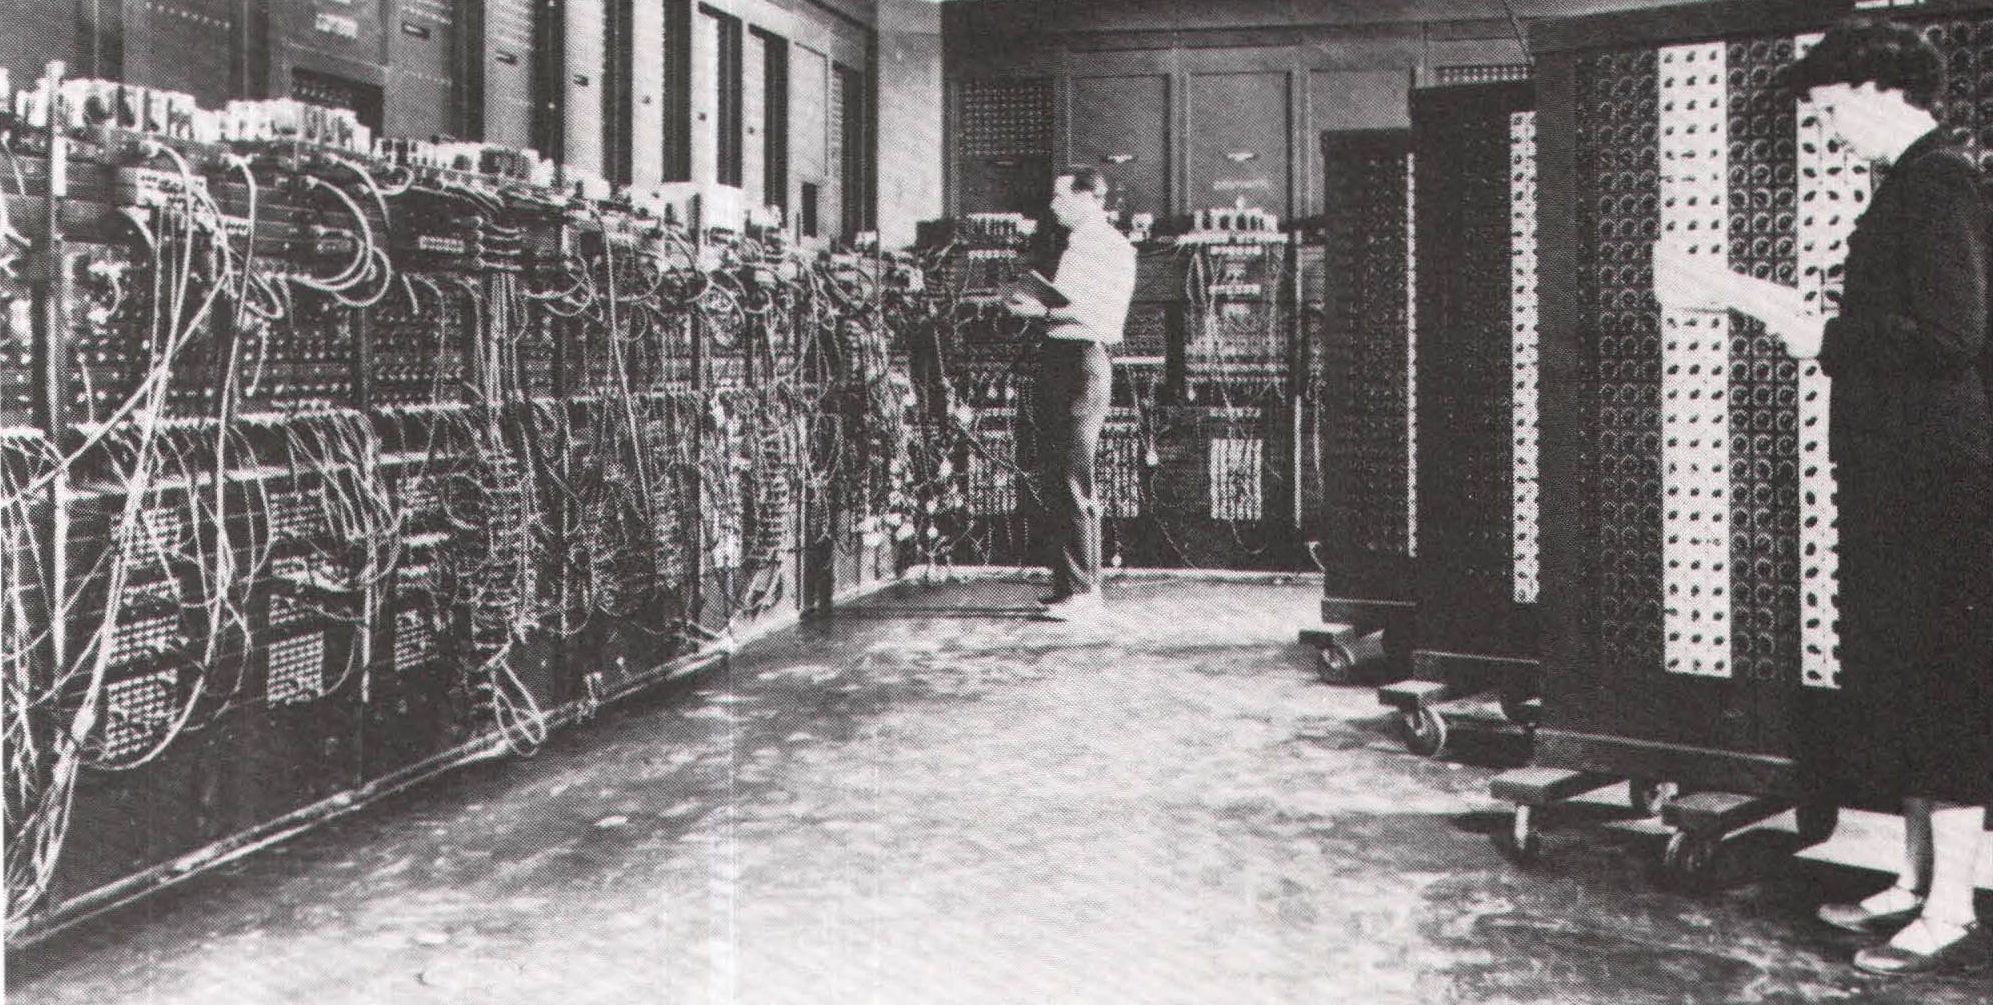
\includegraphics[width=0.5\paperwidth]{resources/eniac}
	\end{figure}
\end{frame}
\begin{frame}{Histórico}
	\framesubtitle{1955-1965}
	\begin{itemize}
		\item Uso de transistores
		\item Máquinas chamadas de \textit{mainframes}
		\item Custo de milhões de dólares
		\item Uso de cartões perfurados
	\end{itemize}
	\begin{figure}
		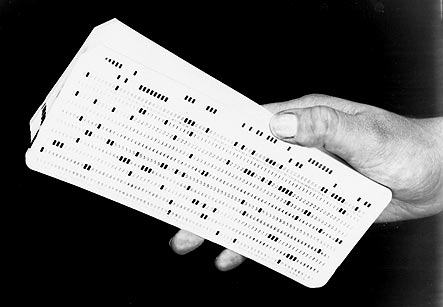
\includegraphics[width=0.5\paperwidth]{resources/punchcards}
	\end{figure}
\end{frame}
\begin{frame}{Histórico}
	\framesubtitle{1955-1965}
	\begin{itemize}
		\item Introdução do conceito de \alert{lotes}
		\item Primeiros ancestrais dos sistemas operacionais modernos
	\end{itemize}
	\begin{figure}
		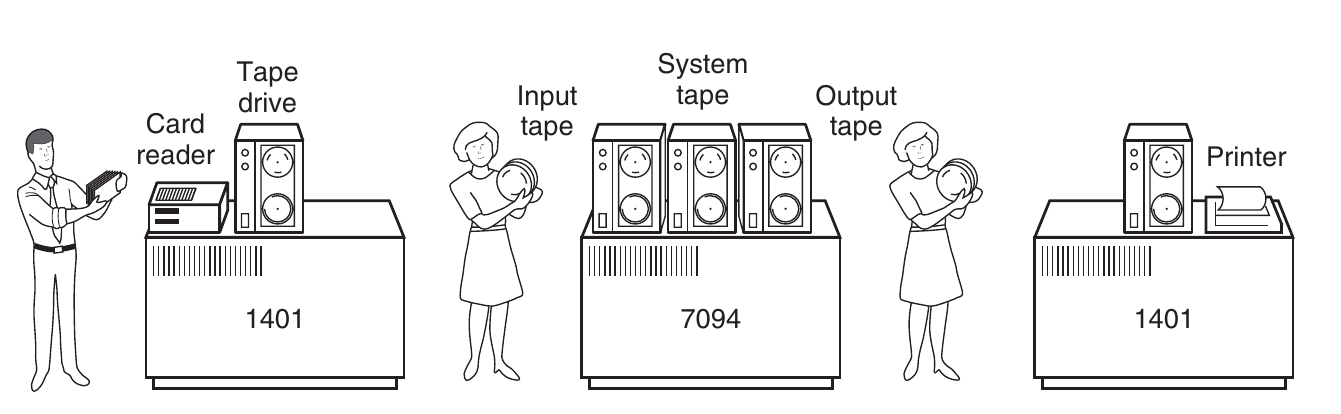
\includegraphics[width=0.8\paperwidth]{resources/batch}
	\end{figure}
\end{frame}
\begin{frame}{Histórico}
	\framesubtitle{1965-1980}
	\begin{itemize}
		\item Introdução de circuitos integrados
		\item IBM 360: primeira família de computadores compatíveis entre si
		\item Sistema operacional único (OS/360): muitos bugs
	\end{itemize}
	\begin{figure}
		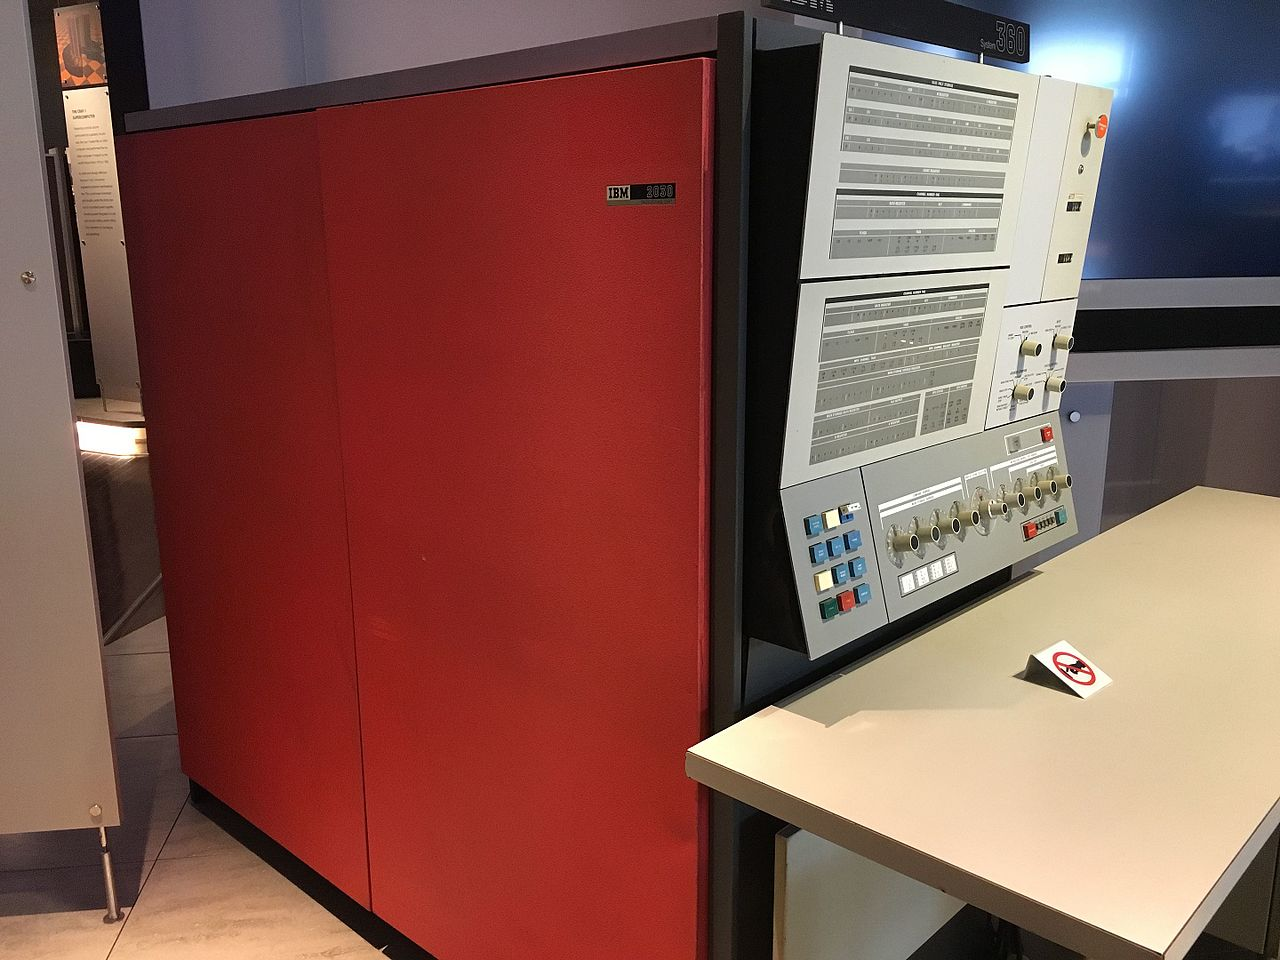
\includegraphics[width=0.5\paperwidth]{resources/ibm360}
	\end{figure}
\end{frame}
\begin{frame}{Histórico}
	\framesubtitle{1965-1980}
	\begin{itemize}
		\item \textbf{Multiprogramação:} enquanto um job faz I/O, outro utiliza a CPU
		\item \textbf{Spooling:} ler jobs dos cartões para o disco imediatamente
		\item Demora entre a entrega do job e a obteção do resultado
	\end{itemize}
	\begin{figure}
		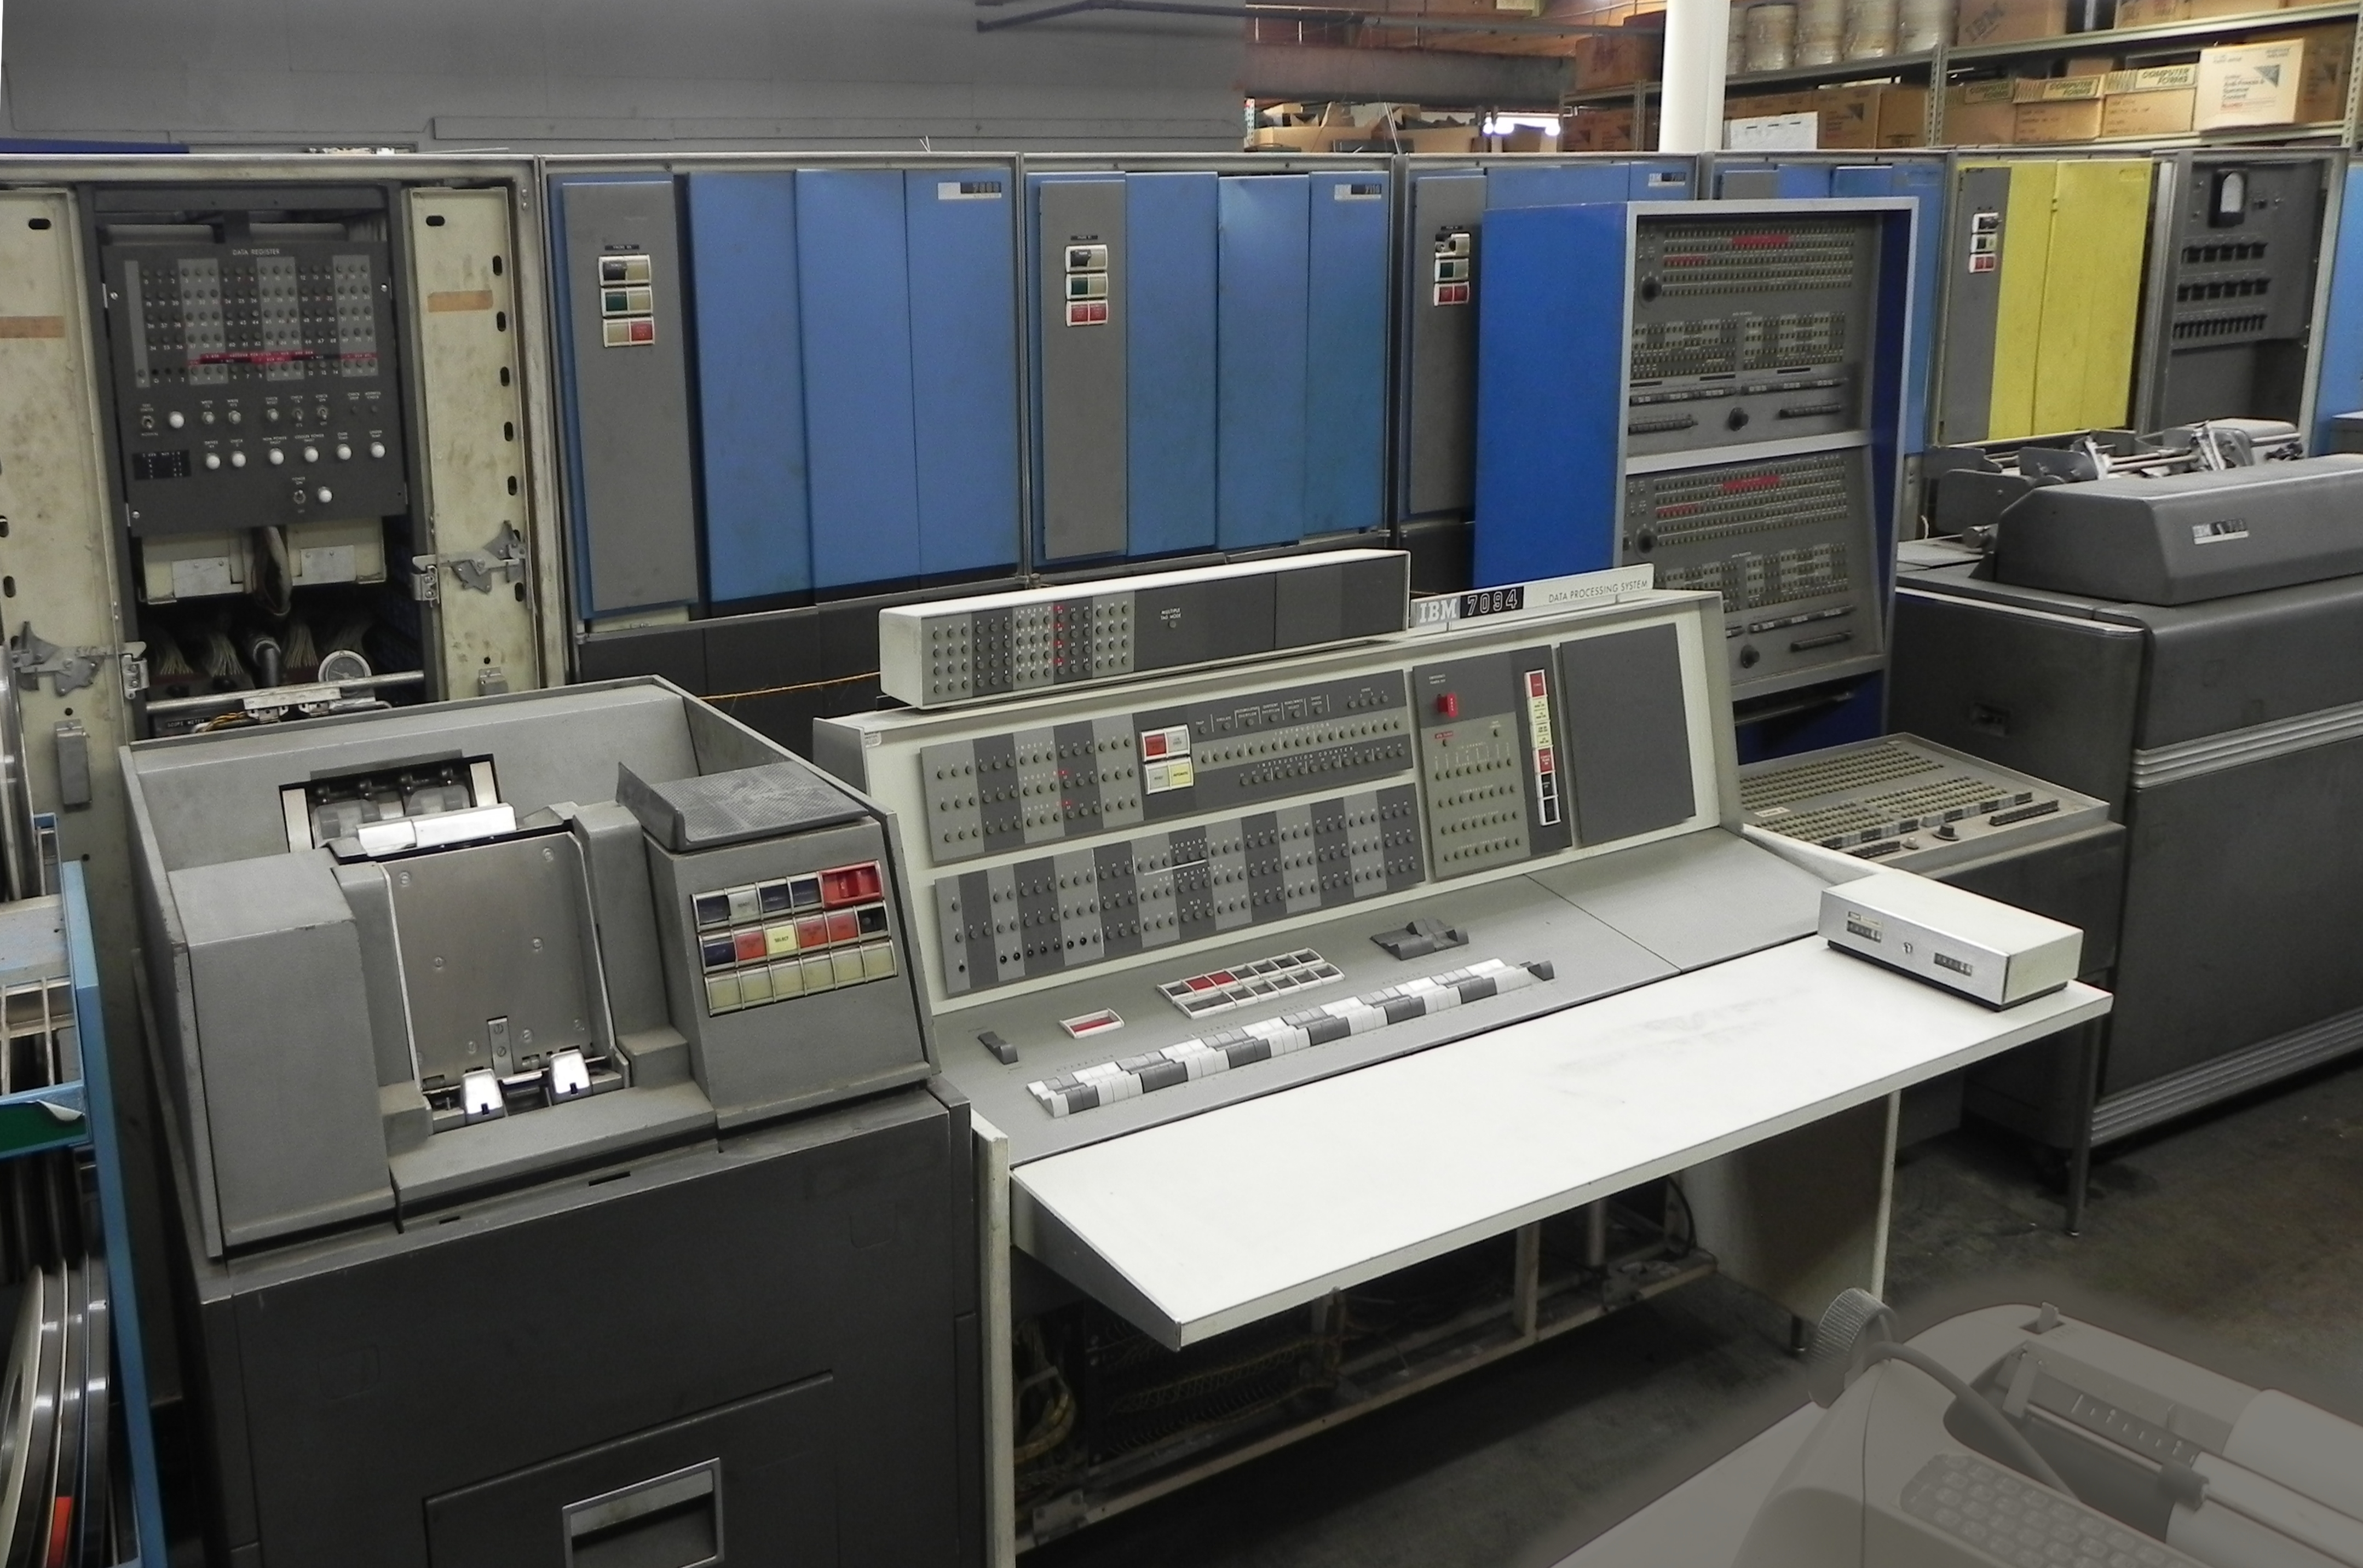
\includegraphics[width=0.5\paperwidth]{resources/ibm7094}
	\end{figure}
\end{frame}
\begin{frame}{Histórico}
	\framesubtitle{1965-1980}
	\begin{itemize}
		\item \textbf{CTSS:} introduziu o conceito de \alert{timesharing}
		\item Usuários conectados simultaneamente através de terminais
		\item CPU executa comandos do usuário e utiliza o tempo ocioso para executar jobs maiores
	\end{itemize}
	\begin{figure}
		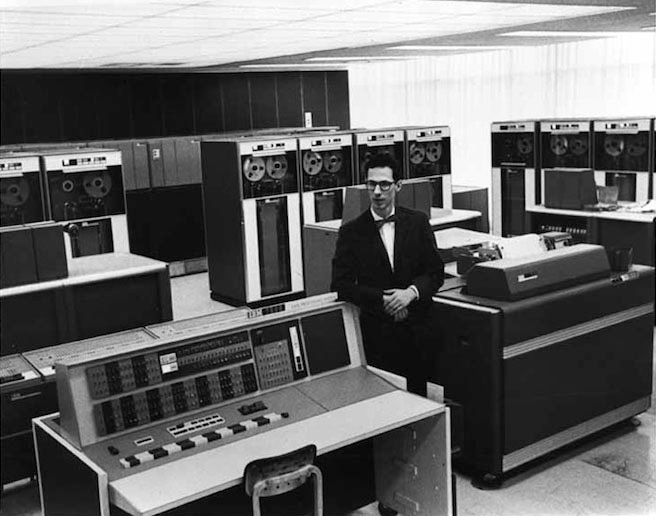
\includegraphics[width=0.4\paperwidth]{resources/ctss}
	\end{figure}
\end{frame}
\begin{frame}{Histórico}
	\framesubtitle{1965-1980}
	\begin{itemize}
		\item \textbf{MULTICS:} um único computador atendendo a centenas de usuários
		\item Pouco sucesso
		\item Má escolha da linguagem (PL/I)
		\item Influenciou diversos sistemas que vieram depois
		\item Hoje uma ideia semelhante ganha força: \alert{computação em nuvem}
	\end{itemize}
	\begin{figure}
		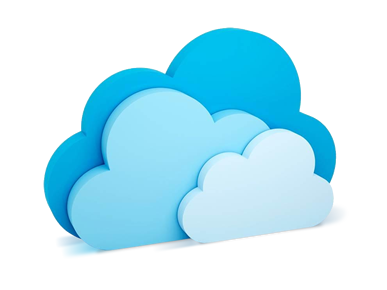
\includegraphics[width=0.4\paperwidth]{resources/cloud}
	\end{figure}
\end{frame}
\begin{frame}{Histórico}
	\framesubtitle{1965-1980}
	\begin{itemize}
		\item Crescimento dos mini-computadores
		\item \textbf{DEC PDP-1:} 120 mil dólares
	\end{itemize}
	\begin{figure}
		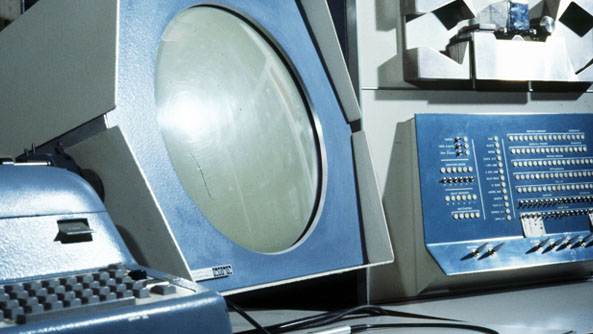
\includegraphics[width=0.5\paperwidth]{resources/pdp1}
	\end{figure}
	\pause
	\begin{tikzpicture}[overlay, remember picture]
	\node[anchor=north east, yshift=-40, xshift=-20] at (current page.north east) {
		
\includegraphics[width=0.3\paperwidth]{resources/shutup}
	};
	\end{tikzpicture}
\end{frame}
\begin{frame}{Histórico}
	\framesubtitle{1965-1980}
	\begin{itemize}
		\item \textbf{Ken Thompson:} usando um PDP-7 da Bell Labs, desenvolveu uma versão do MULTICS para um usuário: \alert{UNIX}
		\item Com o código fonte disponível, empresas desenvolveram suas próprias versões do UNIX:
		\begin{itemize}
			\item[System V] desenvolvido pela AT\&T
			\item[BSD] desenvolvido pela Universidade da Califórnia, em Berkley
		\end{itemize}
	\end{itemize}
	\begin{figure}
		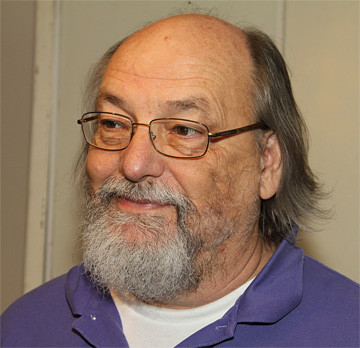
\includegraphics[width=0.3\paperwidth]{resources/thompson}
	\end{figure}
\end{frame}
\begin{frame}{Histórico}
	\framesubtitle{1965-1980}
	\begin{itemize}
		\item Diversas versões do UNIX incompatíveis entre si
		\item \textbf{POSIX:} padrão desenvolvido pelo IEEE que as versões do UNIX devem seguir
		\item{MINIX:} clone do UNIX para fins educacionais desenvolvido por Tanenbaum
		\begin{itemize}
			\item Focado em alta confiabilidade
			\item Substituição de hardware sem necessidade de reiniciar
		\end{itemize}
	\end{itemize}
	\begin{figure}
		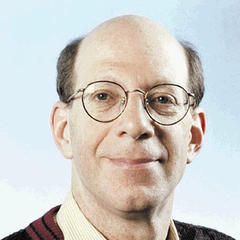
\includegraphics[width=0.2\paperwidth]{resources/tanenbaum}
	\end{figure}
\end{frame}
\begin{frame}{Histórico}
	\framesubtitle{1965-1980}
	\begin{itemize}
		\item \textbf{Linus Torvalds:} criou o \alert{Linux} como uma alternativa gratuita ao MINIX
	\end{itemize}
	\begin{figure}
		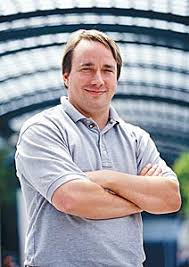
\includegraphics[width=0.3\paperwidth]{resources/linus}
	\end{figure}
	\begin{tikzpicture}[overlay, remember picture]
		\node[anchor=south east, yshift=20, xshift=-20] at (current page.south east) {
			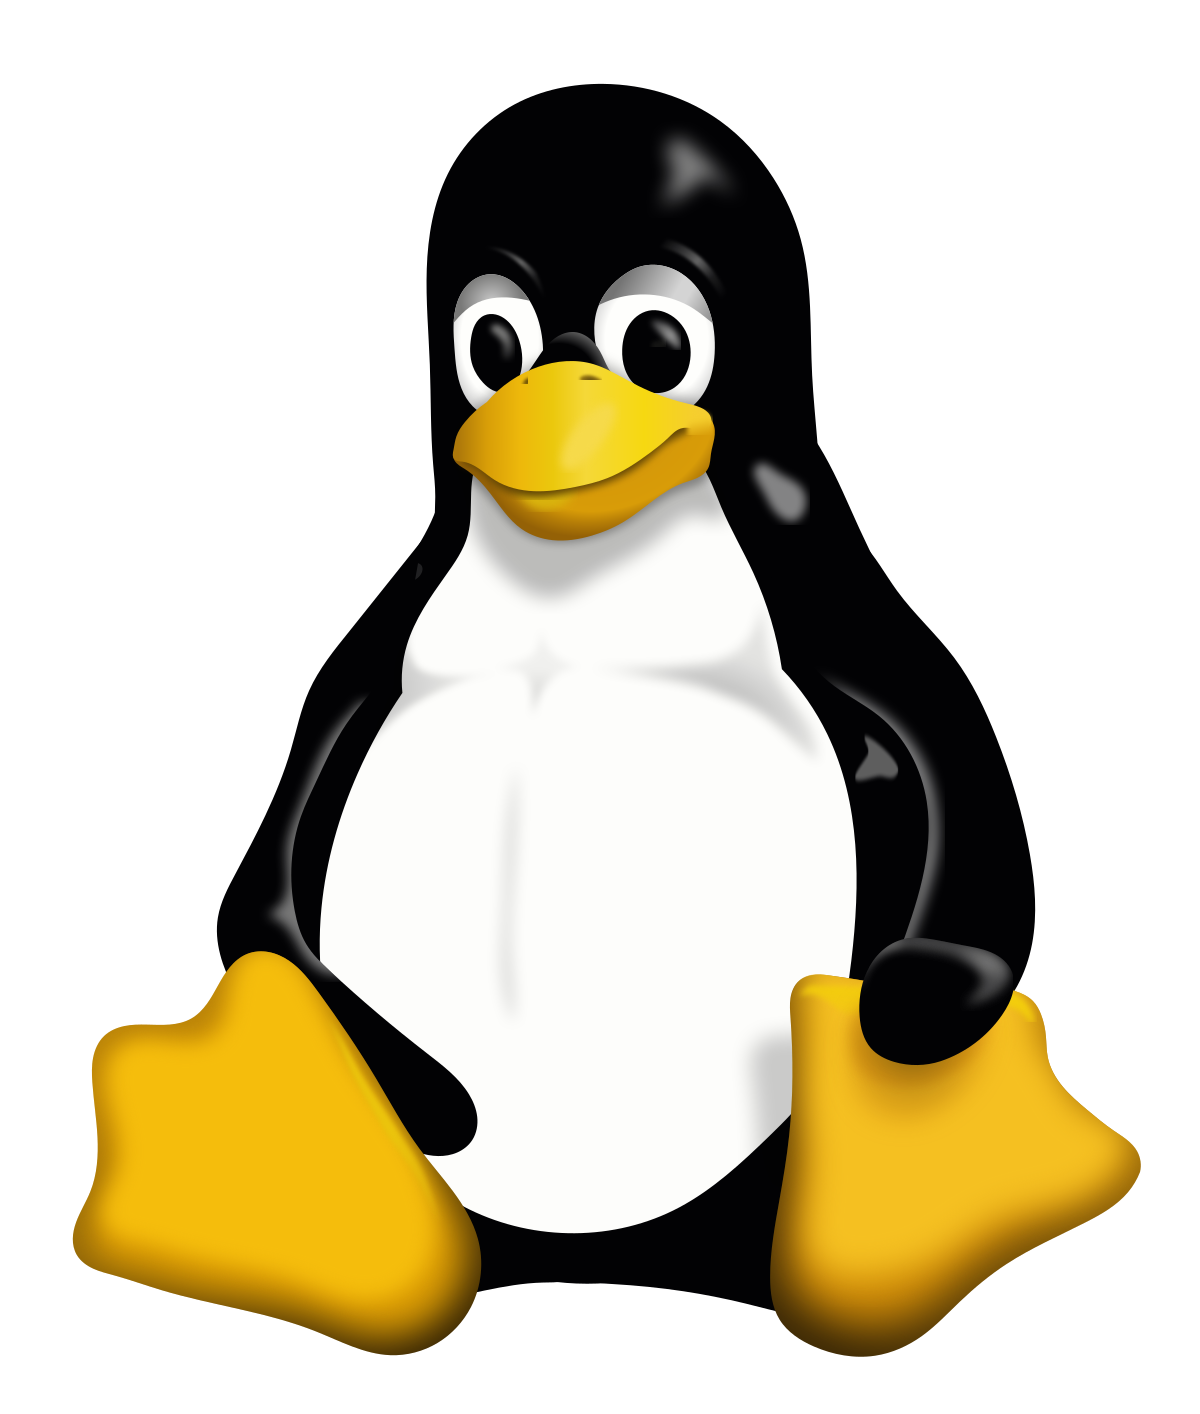
\includegraphics[width=0.2\paperwidth]{resources/tux}
		};
	\end{tikzpicture}
\end{frame}
\begin{frame}{Histórico}
	\framesubtitle{1965-1980}
	\begin{figure}
		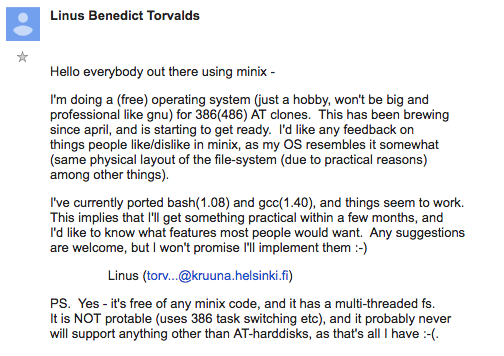
\includegraphics[width=0.7\paperwidth]{resources/linusemail}
	\end{figure}
\end{frame}
\begin{frame}{Histórico}
	\framesubtitle{1965-1980}
	\begin{figure}
		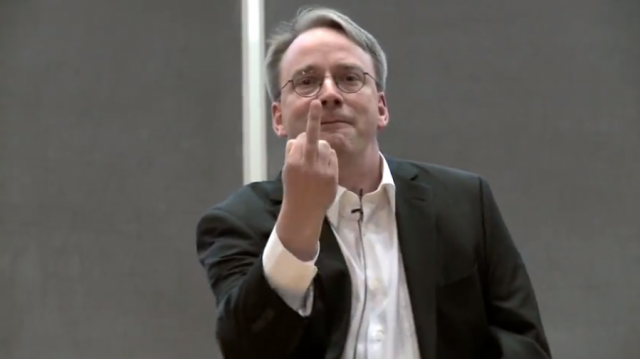
\includegraphics[width=0.7\paperwidth]{resources/linus2}
	\end{figure}
\end{frame}
\begin{frame}{Histórico}
	\framesubtitle{1980-presente}
	\begin{itemize}
		\item Circuitos integrados em larga escala deram origem aos \alert{microcomputadores}
		\item Início da era dos computadores pessoais
		\item \textbf{Gary Kildall:} criou o \alert{CP/M} para a Intel
	\end{itemize}
	\begin{figure}
		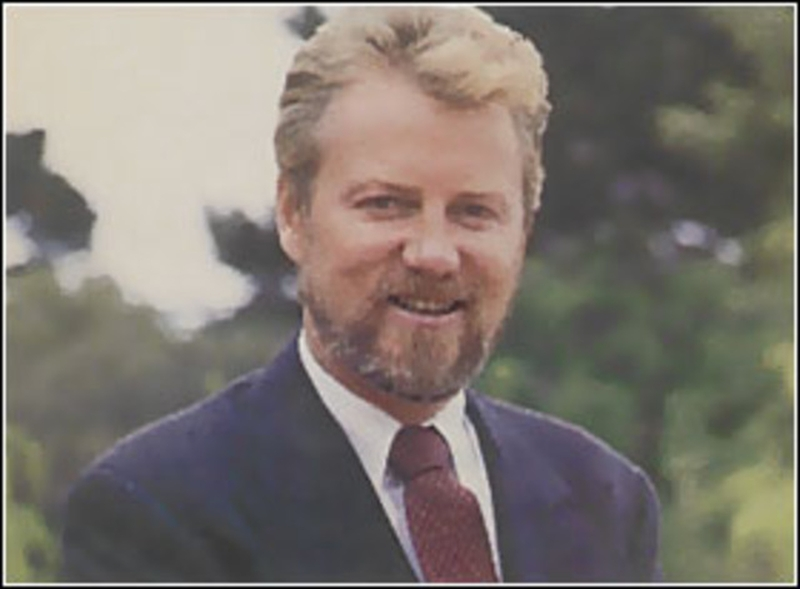
\includegraphics[width=0.4\paperwidth]{resources/gary}
	\end{figure}
\end{frame}
\begin{frame}{Histórico}
	\framesubtitle{1980-presente}
	\only<1>{
		\begin{itemize}
			\item Intel não viu futuro em computadores baseados em disco
			\item Kildall pediu os direitos do CP/M e fundou a Digital Research
			\item Dominou o mercado por certa de 5 anos
			\item IBM estava desenvolvendo o IBM-PC nos anos 80
			\item Entraram em contato com Bill Gates para licensiar seu interpretador de BASIC
		\end{itemize}
		\begin{figure}
			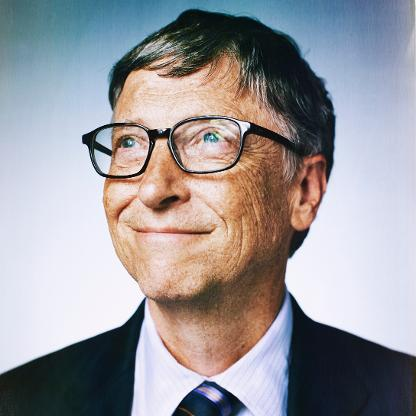
\includegraphics[width=0.25\paperwidth]{resources/gates}
		\end{figure}
	}
	\only<2>{
		\begin{itemize}
			\item Pediram a Gates uma recomendação de um sistema operacional
			\item Ele indicou a Digital Research
			\item Kildall se recusou a falar com a IBM e enviou um subordinado
			\item Também recusou-se a assinar o NDA em relação ao IBM-PC
		\end{itemize}
	}
	\only<3>{
		\begin{itemize}
			\item A IBM pediu a Gates que produzisse um sistema operacional
			\item Gates comprou o \textbf{Disk Operating System - DOS} de um fabricante de computadores local
			\item Gates contratou Tim Paterson, o criador do DOS, para realizar modificações no sistema, que foi chamado de \textbf{Microsoft DOS (MS-DOS)}
			\item Tempos depois, Kildall morreu de causas desconhecidas
		\end{itemize}
	}
	\begin{tikzpicture}[overlay, remember picture]
	\node[anchor=north east, yshift=-5, xshift=-20] at (current page.north east) {
		
\includegraphics[width=0.6\paperwidth]{resources/casos}
	};
	\end{tikzpicture}
\end{frame}
\begin{frame}{Histórico}
	\framesubtitle{1980-presente}
	\begin{itemize}
		\item \textbf{Doug Engelbart:} inventou a primeira interface gráfica no Stanford Research Institute
		\item Ideias adotadas pelos pesquisadores da Xerox
	\end{itemize}
	\begin{figure}
		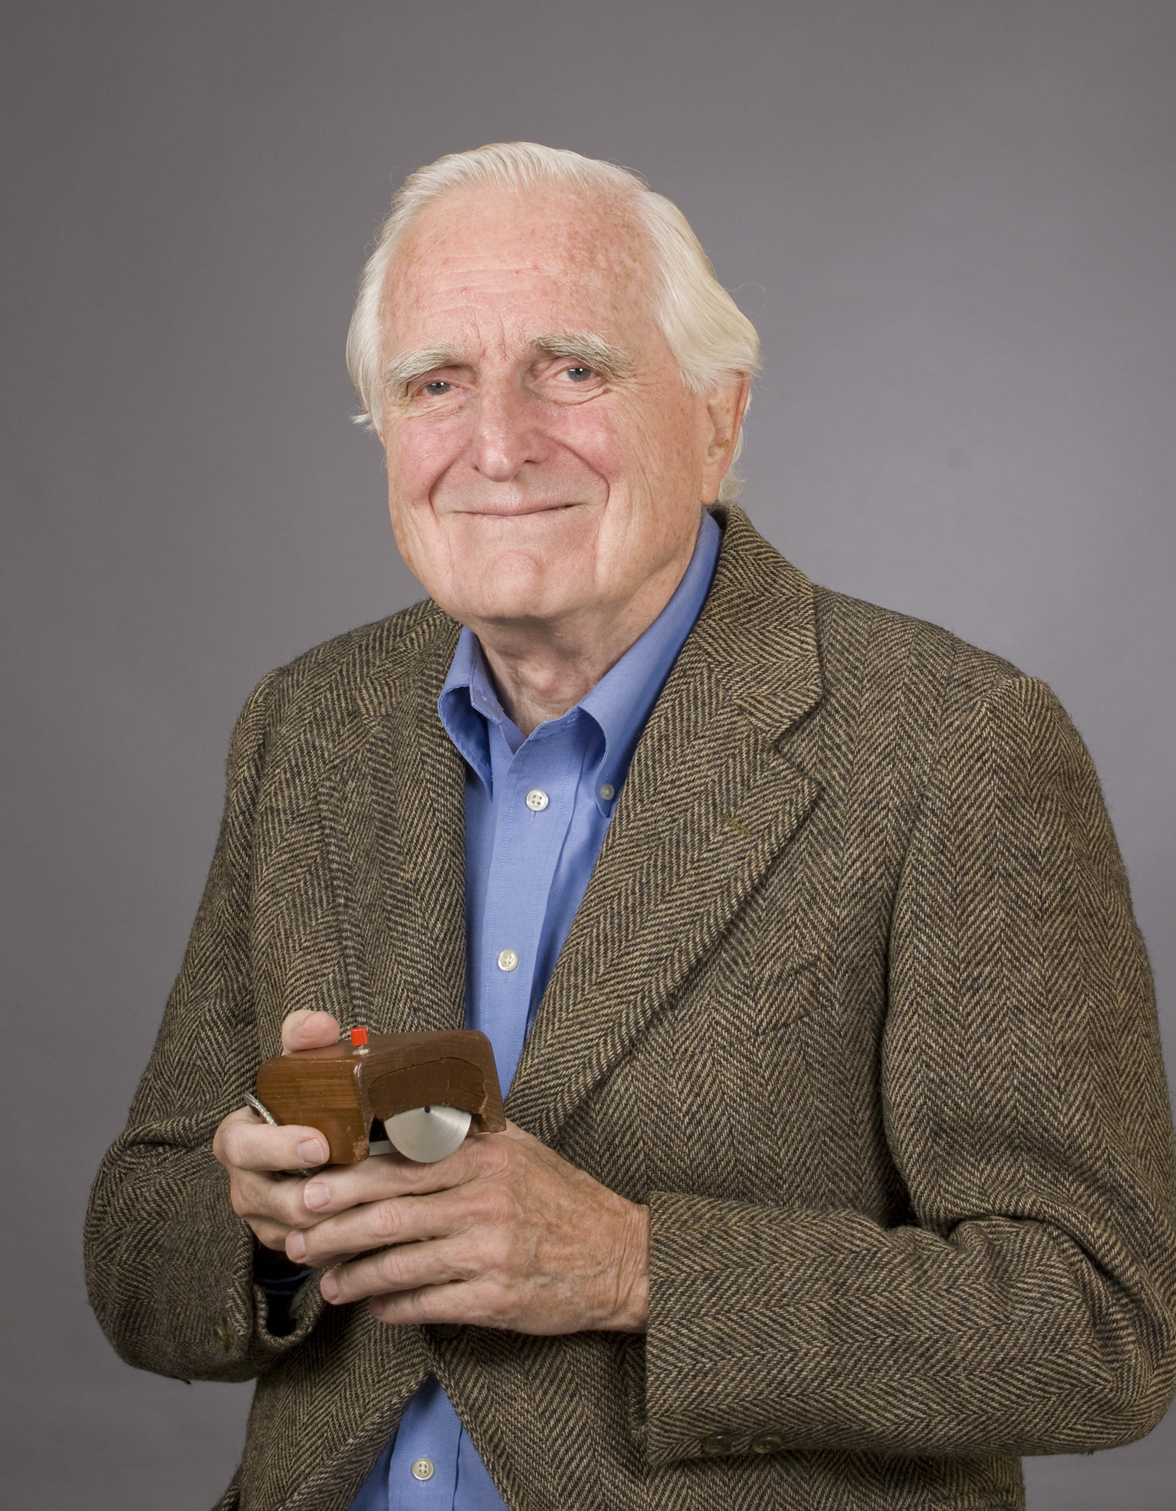
\includegraphics[width=0.3\paperwidth]{resources/doug}
	\end{figure}
\end{frame}
\begin{frame}{Histórico}
	\framesubtitle{1980-presente}
	\begin{itemize}
		\item \textbf{Steve Jobs:} utilizou as ideias da Xerox no Lisa e posteriormente no Apple Macintosh
	\end{itemize}
	\begin{figure}
		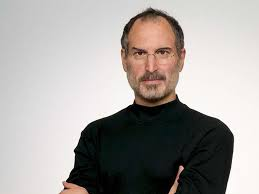
\includegraphics[width=0.4\paperwidth]{resources/jobs}
	\end{figure}
\end{frame}
\begin{frame}{Histórico}
	\framesubtitle{1980-presente}
	\begin{itemize}
		\item Microsoft usou ideias do Macintosh para desenvolver o sucessor do MS-DOS
		\item O \textbf{Windows} era, inicialmente, um ambiente gráfico dentro do MS-DOS
		\item \textbf{Windows 95} incorporou recursos de sistema operacional nele
		\item \textbf{Windows NT} eliminou a dependência com o MS-DOS
	\end{itemize}
	\begin{figure}
		
\includegraphics[width=0.8\paperwidth]{resources/windows}
	\end{figure}
\end{frame}
\begin{frame}{Histórico}
	\framesubtitle{1980-presente}
	\begin{itemize}
		\item A versão 5 do Windows NT foi renomeada para \textbf{Windows 2000} para ser o sucessor do Windows 98 e do Windows NT, mas não fez sucesso
		\item Microsoft criou uma versão do Windows 98 chamada \textbf{Windows Me} (Millennium Edition)
		\item Em 2001, uma versão melhorada do Windows 2000 foi lançada: o \textbf{Windows XP}
	\end{itemize}
	\begin{figure}
		
\includegraphics[width=0.8\paperwidth]{resources/windows}
	\end{figure}
\end{frame}
\begin{frame}{Histórico}
	\framesubtitle{1980-presente}
	\begin{itemize}
		\item O sucessor do Windows XP, o \textbf{Windows Vista} foi lançado em 2007
		\item Com o pouco sucesso do Vista, em seguida foi lançado o \textbf{Windows 7}
		\item Em 2012, foi lançado o \textbf{Windows 8}, com uma nova interface voltada a telas de toque
		\item A versão atual do sistema é o \textbf{Windows 10}, chamado pela Microsoft de \alert{o último Windows}
	\end{itemize}
	\begin{figure}
		
\includegraphics[width=0.8\paperwidth]{resources/windows}
	\end{figure}
\end{frame}
\begin{frame}{Histórico}
	\framesubtitle{Dispositivos móveis}
	\begin{itemize}
		\item Primeiro telefone móvel surgiu em 1946 e pesava 40 quilos

	\end{itemize}
	\begin{figure}
		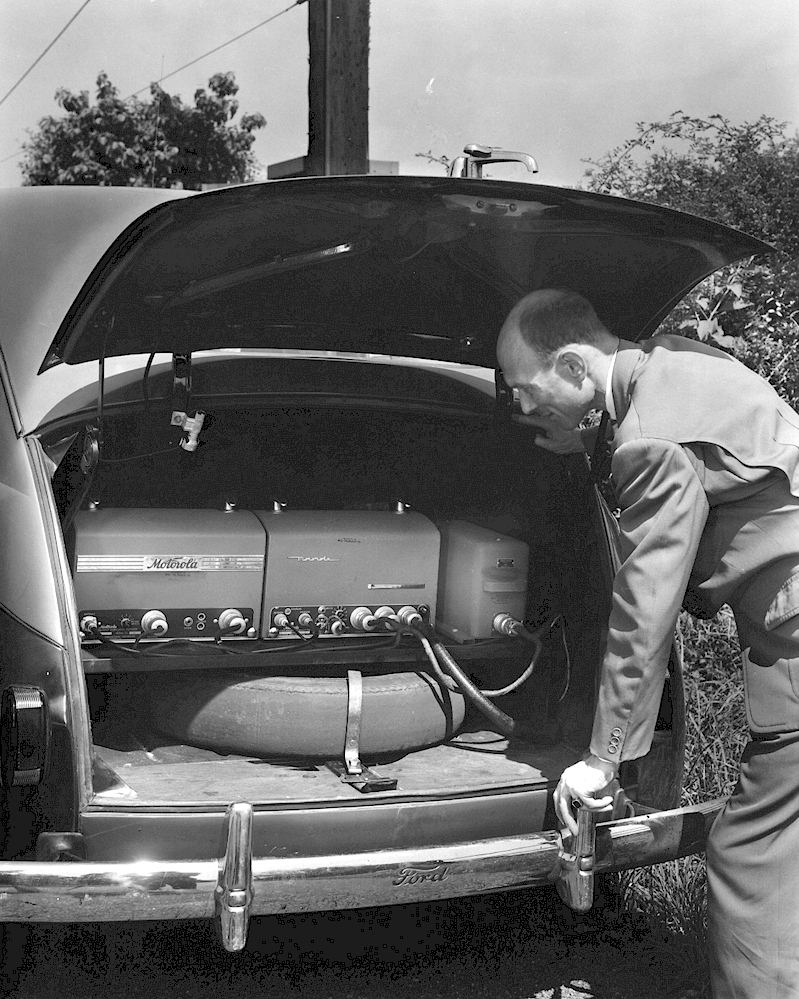
\includegraphics[width=0.35\paperwidth]{resources/movel}
	\end{figure}
\end{frame}
\begin{frame}{Histórico}
	\framesubtitle{Dispositivos móveis}
	\begin{itemize}
		\item Nos anos 70, surgiu o primeiro ``tijolão'', pesando cerca de um quilo
		
	\end{itemize}
	\begin{figure}
		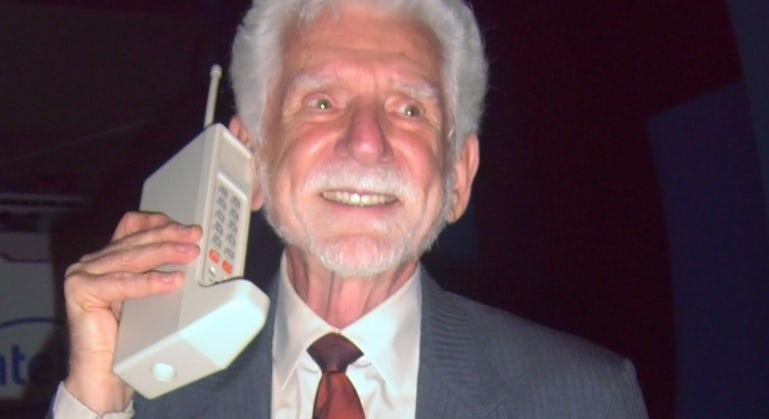
\includegraphics[width=0.6\paperwidth]{resources/tijolao}
	\end{figure}
\end{frame}
\begin{frame}{Histórico}
	\framesubtitle{Dispositivos móveis}
	\begin{itemize}
		\item O primeiro smartphone surgiu no meio dos anos 90: o Nokia N9000
		\item O termo \textbf{smartphone} foi cunhado pela Ericsson em 1997 para o GS88 `Penelope'
	\end{itemize}
	\begin{tikzpicture}
	\node (n9000) at (0,0) {
		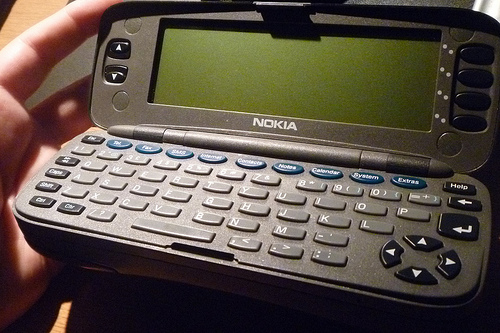
\includegraphics[width=0.4\paperwidth]{resources/n9000}
	};
	\node[right=of n9000] (gs88) {
		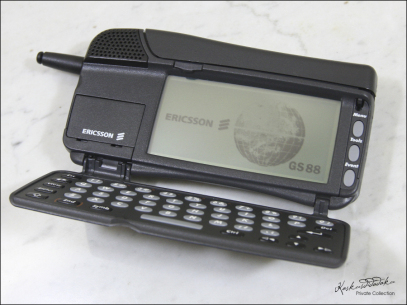
\includegraphics[width=0.3\paperwidth]{resources/gs88}
	};
	\end{tikzpicture}
\end{frame}
\begin{frame}{Histórico}
	\framesubtitle{Dispositivos móveis}
	\begin{itemize}
		\item No início, o sistema mais popular era o \textbf{Symbian OS}
		\item Hoje, o \textbf{Android} domina o mercado, com o \textbf{iOS} em segundo lugar
	\end{itemize}
	\begin{figure}
		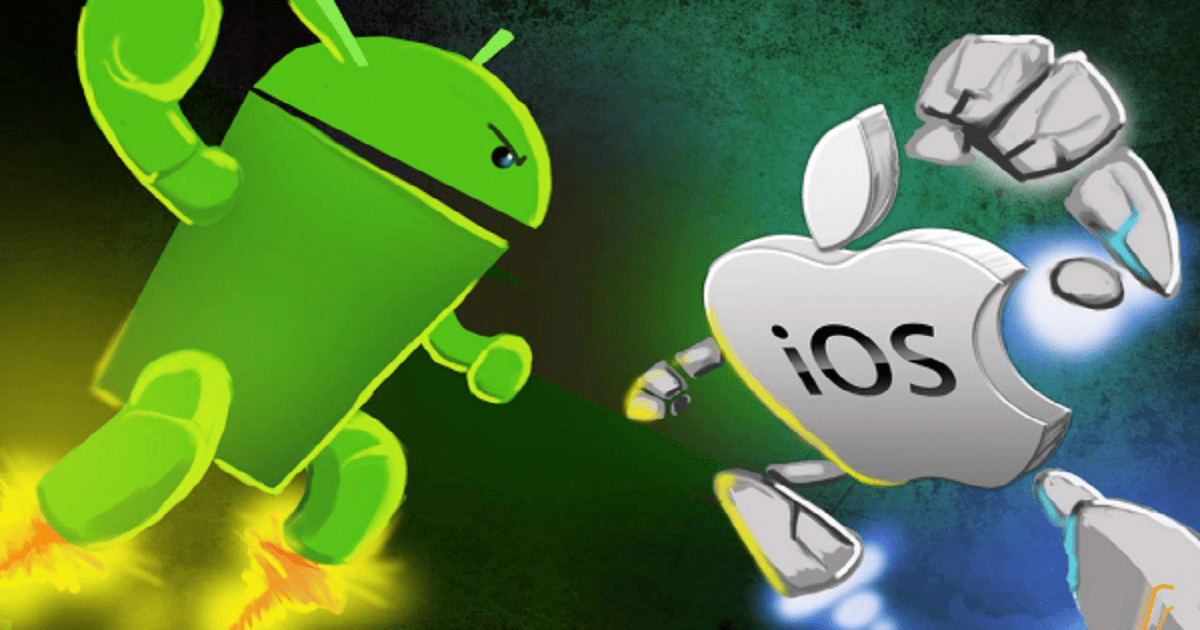
\includegraphics[width=0.6\paperwidth]{resources/android-ios}
	\end{figure}
\end{frame}

\section{Revisão: hardware}
\begin{frame}{Revisão: hardware}
	\framesubtitle{Processadores}
	\begin{itemize}
		\item ``Cérebro'' do computador
		\item Chamado de \alert{CPU}
		\item Operação básica:
		\begin{itemize}
			\item Obtem instrução da memória
			\item Decodifica a instrução
			\item Executa a instrução
		\end{itemize}
		\item Cada CPU tem um \alert{conjunto de instruções} próprio
	\end{itemize}
	\begin{figure}
		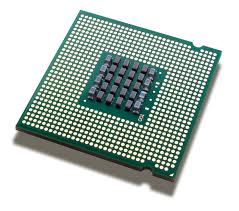
\includegraphics[width=0.3\paperwidth]{resources/processor}
	\end{figure}
\end{frame}
\begin{frame}{Revisão: hardware}
	\framesubtitle{Processadores}
	\begin{itemize}
		\item \textbf{Registradores} são pequenas memórias dentro do processador
		\item Dados da memória são carregados nos registradores
		\item Demais instruções operam sobre os dados dos registradores
		\item Esses dados são escritos de volta para a memória
		\item Registradores especiais:
			\begin{itemize}
				\item[PC] Program Counter, contém o endereço da próxima instrução
				\item[SP] Stack Pointer, aponta para o endereço do topo da pilha
				\item[PSW] Program Status Word, informações do status atual da CPU
			\end{itemize}
		\item Sistemas operacionais precisam manipular corretamente estes registradores
	\end{itemize}
\end{frame}
\begin{frame}{Revisão: hardware}
	\framesubtitle{Processadores}
	\begin{itemize}
		\item Para acelerar a execução, processadores usam \alert{pipelines}
	\end{itemize}
	\begin{center}
		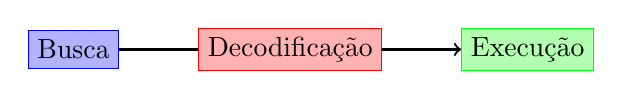
\begin{tikzpicture}[node distance=3mm and 1cm]
		\centering
		\node[draw=blue, fill=blue!30] (busca) at (0,0) {Busca};
		\node[draw=red, fill=red!30, right=of busca] (decod) {Decodificação};
		\node[draw=green, fill=green!30, right=of decod] (exec) {Execução};
		\draw[->, thick] (busca) -- (decod) -- (exec);
		\end{tikzpicture}
	\end{center}
	\begin{itemize}
		\item Processadores modernos usam pipelines longas (14-16 num Intel Kaby Lake)
		\item \textbf{Spectre} e \textbf{Meltdown}: exploram execução especulativa
	\end{itemize}
	\begin{figure}
		
\includegraphics[width=0.3\paperwidth]{resources/meltdown-spectre}
	\end{figure}
\end{frame}
\begin{frame}{Revisão: hardware}
	\framesubtitle{Processadores}
	\begin{itemize}
		\item Processadores \alert{superescalares} utilizam múltiplas unidades de execução (ex: uma para inteiros, uma para float, uma para booleano)
		\item Execução fora de ordem
	\end{itemize}
	\begin{center}
		\begin{tikzpicture}[node distance=1cm]
		\centering
		\node[draw=blue, fill=blue!30] (busca1) at (0,0) {Busca};
		\node[draw=red, fill=red!30, right=of busca1] (decod1) {Decodificação};
		\node[draw=blue, fill=blue!30, below=of busca1] (busca2) at (0,0) {Busca};
		\node[draw=red, fill=red!30, right=of busca2] (decod2) {Decodificação};
		\node[draw=orange, fill=orange!30, right=of decod] (buffer) {Buffer};
		\node[draw=green, fill=green!30, right=of buffer] (exec1) {Execução};
		\node[draw=green, fill=green!30, below=of exec1] (exec2) {Execução};
		\node[draw=green, fill=green!30, below=of exec2] (exec3) {Execução};
		\draw[->, thick] (busca1) -- (decod1) -- (buffer);
		\draw[->, thick] (busca2) -- (decod2) -- (buffer);
		\draw[->, thick] (buffer) -- (exec1);
		\draw[->, thick] (buffer) -- (exec2);
		\draw[->, thick] (buffer) -- (exec3);
		\end{tikzpicture}
	\end{center}
\end{frame}
\begin{frame}{Revisão: hardware}
	\framesubtitle{Processadores}
	\begin{itemize}
		\item A maioria das CPUs possui dois \alert{modos de operação}
		\begin{itemize}
			\item[Modo kernel] Possui acesso a todas as instruções da CPU. O sistema operacional roda neste modo
			\item[Modo usuário] Algumas instruções não estão acessíveis. Demais programas rodam neste modo
		\end{itemize}
		\item Usa-se um bit na PSW para mudar de um modo para outro
		\item Um programa usa serviços do sistema operacional por meio de \alert{chamadas de sistema}
		\item Chamadas de sistema entram em modo kernel e invocam o sistema operacional
		\item Ao final da chamada, o programa volta a executar em modo usuário
	\end{itemize}
\end{frame}
\begin{frame}{Revisão: hardware}
	\framesubtitle{Multithread e multicore}
	\begin{itemize}
		\item \textbf{Lei de Moore:} o número de transistores em um chip dobra a cada 18 meses
	\end{itemize}
	\begin{figure}
		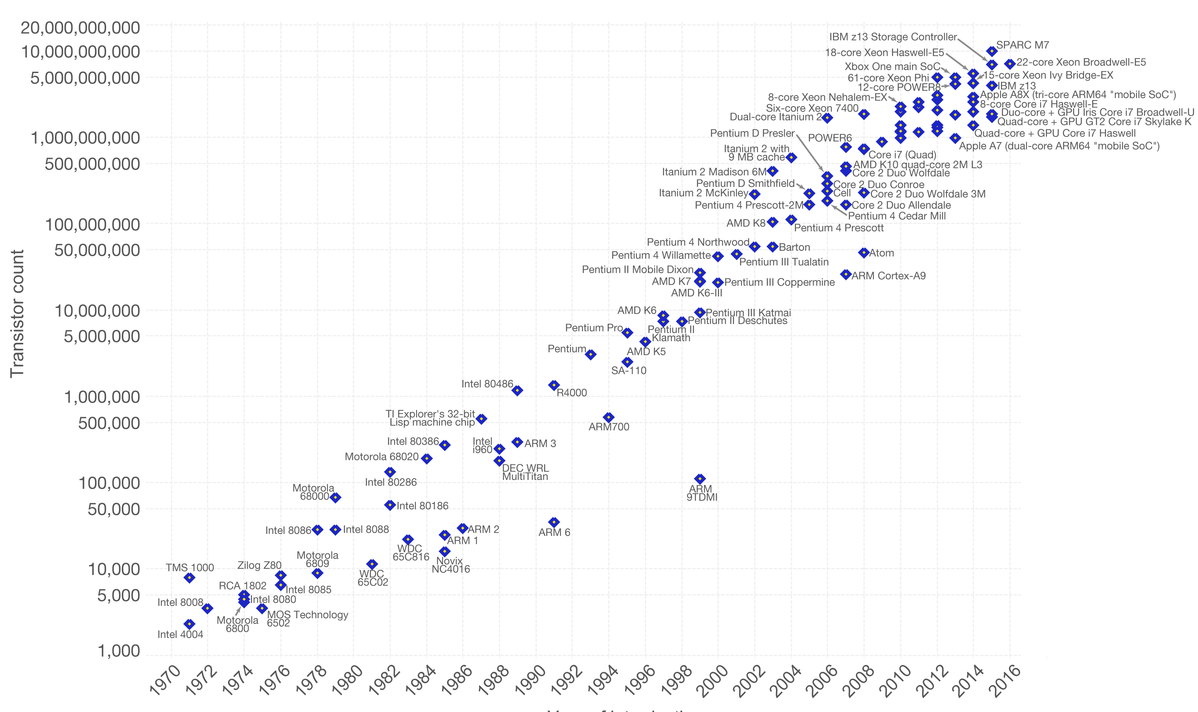
\includegraphics[width=0.7\paperwidth]{resources/moore}
	\end{figure}
\end{frame}
\begin{frame}{Revisão: hardware}
	\framesubtitle{Multithread e multicore}
	\begin{itemize}
		\item O que fazer com tantos transistores?
		\item \textbf{Multithreading} ou \textbf{Hyperthreading}:
		\begin{itemize}
			\item Armazenar o estado de duas threads
			\item Troca extremamente rápida entre elas
			\item Aparece para o sistema operacional como dois processadores
			\item Não é paralelismo real
		\end{itemize}
		\item Múltiplos núcleos (cores):
		\begin{itemize}
			\item Múltiplos processadores dentro do mesmo chip
			\item Paralelismo real
		\end{itemize}
	\end{itemize}
\end{frame}
\begin{frame}{Revisão: hardware}
	\framesubtitle{Memória}
	\begin{itemize}
		\item Memória ideal:
		\begin{itemize}
			\item Extremamente rápida
			\item Extremamente grande
			\item Extremamente barata
		\end{itemize}
		\item Nenhuma tecnologia atende a todos esses requisitos
		\item Solução: níveis de memória
		\begin{figure}
			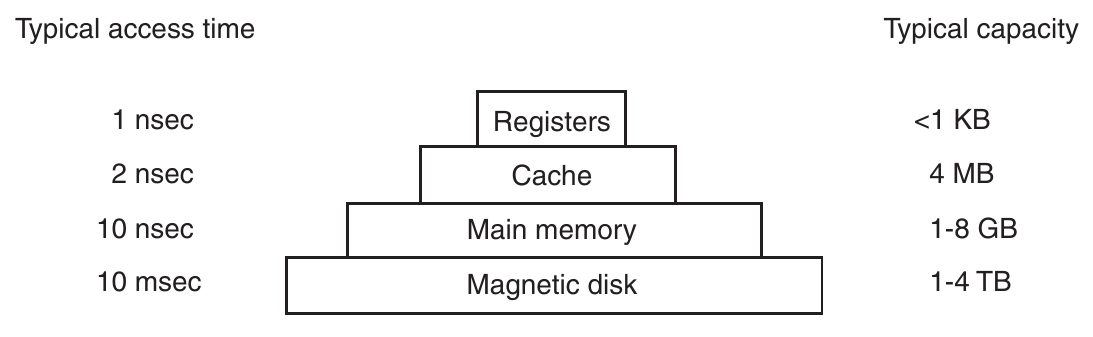
\includegraphics[width=0.7\paperwidth]{resources/niveismem}
		\end{figure}
	\end{itemize}
\end{frame}
\begin{frame}{Revisão: hardware}
	\framesubtitle{Memória}
	\begin{itemize}
		\item Registradores:
		\begin{itemize}
			\item Feitos do mesmo material da CPU
			\item Extremamente rápidos
			\item Poucos disponíveis
			\item Programas devem decidir o que manter nos registradores
		\end{itemize}
		\item Cache:
		\begin{itemize}
			\item Memória rápida e cara
			\item Quando a CPU acessa um dado, ele é buscado no cache
			\item \textbf{Cache hit:} dado encontrado no cache
			\item \textbf{Cache miss:} dado não encontrado será buscado da memória
		\end{itemize}
	\end{itemize}
\end{frame}
\begin{frame}{Revisão: hardware}
	\framesubtitle{Memória}
	\begin{itemize}
		\item Caches geralmente são divididos em níveis
		\item Dados acessados mais frequentemente ficam nos caches mais rápidos
		\begin{itemize}
			\item[Cache L1] Fica dentro da CPU. Tem apenas alguns quilobytes e é o cache mais rápido
			\item[Cache L2] Tem alguns megabytes. Pode ficar dentro do processador ou ser compartilhado pelos núcleos
		\end{itemize}
		\begin{figure}
			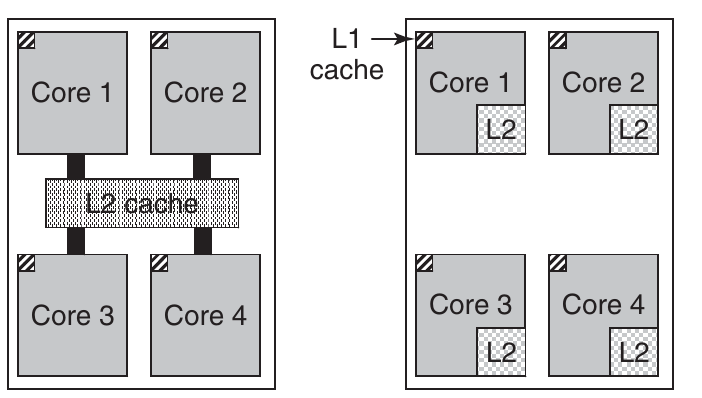
\includegraphics[width=0.5\paperwidth]{resources/cache}
		\end{figure}
	\end{itemize}
\end{frame}
\begin{frame}{Revisão: hardware}
	\framesubtitle{Memória}
	\begin{itemize}
		\item Random Access Memory (RAM)
		\begin{itemize}
			\item Memória principal do computador
			\item Dados não encontrados no cache são buscados na RAM
		\end{itemize}
		\begin{figure}
			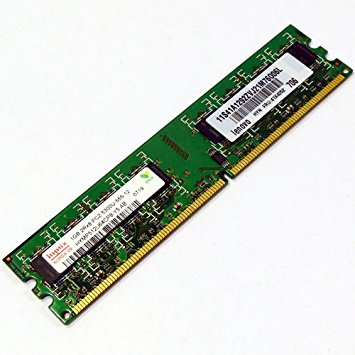
\includegraphics[width=0.4\paperwidth]{resources/memory}
		\end{figure}
	\end{itemize}
\end{frame}
\begin{frame}{Revisão: hardware}
	\framesubtitle{Memória}
	\begin{itemize}
		\item Read-Only Memory (ROM)
		\begin{itemize}
			\item Memória somente para leitura
			\item Presente em pequenas quantidades
			\item Rápida e barata
			\item Não perde os dados ao ser apagada
			\item Geralmente armazena códigos usados na inicialização do computador
		\end{itemize}
		\item Electrically Erasable PROM (EEPROM) e memória flash:
		\begin{itemize}
			\item Mantém os dados ao serem desligadas
			\item Escrita muito mais lenta que em RAM
			\item Geralmente utilizadas no lugar de ROMs (permitem modificação)
			\item Também utilizada em cartões de memória
		\end{itemize}
		\item Memória CMOS
		\begin{itemize}
			\item Utiliza pouquíssima energia para manter os dados
			\item Armazena informações como o relógio e configurações
		\end{itemize}
	\end{itemize}
\end{frame}
\begin{frame}{Revisão: hardware}
	\framesubtitle{Discos}
	\begin{itemize}
		\item Próximo nível na hierarquia de memória
		\item Comparação com RAM:
		\begin{itemize}
			\item 100x mais baratos
			\item 100x maiores
			\item 1000x mais lentos
		\end{itemize}
	\end{itemize}
	\begin{figure}
		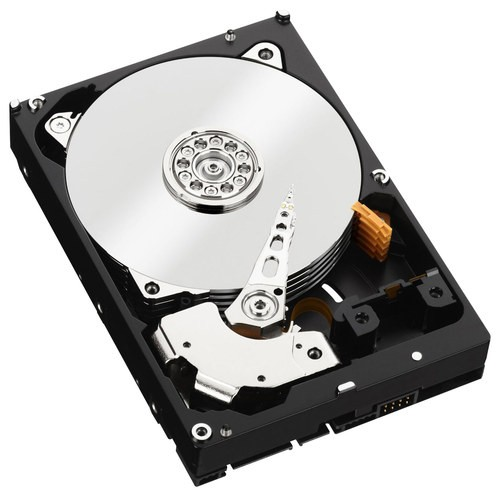
\includegraphics[width=0.3\paperwidth]{resources/hd}
	\end{figure}
\end{frame}
\begin{frame}{Revisão: hardware}
	\framesubtitle{Discos}
	\begin{itemize}
		\item Cada disco é composto de regiões circulares chamadas \alert{trilhas (tracks)}
		\item As trilhas em uma determinada posição do braço formam um \alert{cilindro}
		\item Cada trilha é dividida em \alert{setores} (geralmente de 512 bytes)
		
	\end{itemize}
	\begin{figure}
		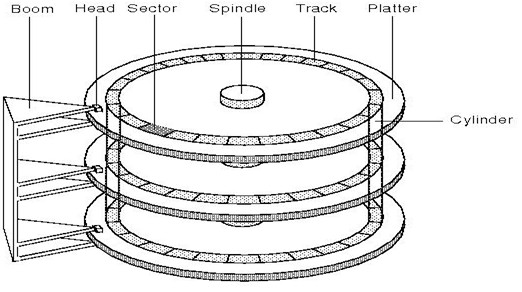
\includegraphics[width=0.5\paperwidth]{resources/cylinder}
	\end{figure}
\end{frame}
\begin{frame}{Revisão: hardware}
	\framesubtitle{Discos}
	\begin{itemize}
		\item Solid State Disks (SSDs):
		\begin{itemize}
			\item Utilizam memória flash
			\item Não possuem partes móveis
			\item Muito mais rápidos que discos
		\end{itemize}
	\end{itemize}
	\begin{figure}
		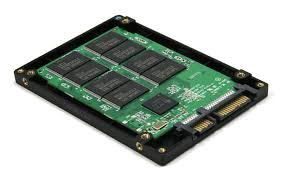
\includegraphics[width=0.5\paperwidth]{resources/ssd}
	\end{figure}
\end{frame}
\begin{frame}{Revisão: hardware}
	\framesubtitle{Dispositivos de entrada e saída (I/O)}
	\begin{itemize}
		\item Diversos tipos de dispositivos interagem com o sistema operacional
	\end{itemize}
	\begin{tikzpicture}[overlay, remember picture]
	\node[anchor=south east, yshift=20, xshift=-20] at (current page.south east) {
		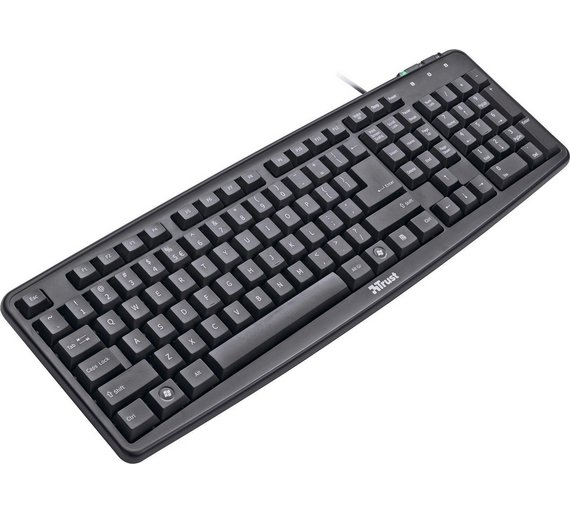
\includegraphics[width=0.3\paperwidth]{resources/keyboard}
	};
	\node[anchor=north east, yshift=-20, xshift=-20] at (current page.north east) {
		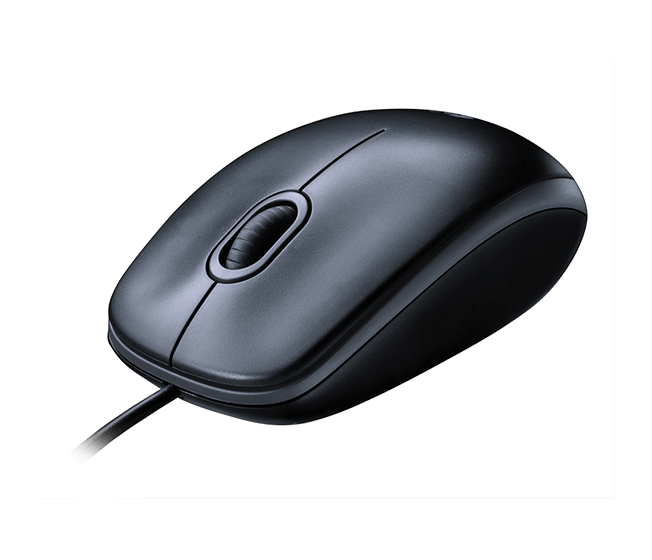
\includegraphics[width=0.2\paperwidth]{resources/mouse}
	};
	\node[anchor=south west, yshift=20, xshift=20] at (current page.south west) {
		\includegraphics[width=0.2\paperwidth]{resources/flashdrive}
	};
	\end{tikzpicture}
\end{frame}
\begin{frame}{Revisão: hardware}
	\framesubtitle{Dispositivos de entrada e saída (I/O)}
	\begin{itemize}
		\item Em geral são compostos de duas partes:
		\begin{itemize}
			\item[Dispositivo] O dispositivo físico
			\item[Controlador] Realiza o controle do dispositivo (que pode ser muito complexo) e oferece uma interface mais simples ao sistema operacional
		\end{itemize}
		\item O sistema operacional se comunica com os dispositivos por meio de \alert{drivers} (fornecidos pelo fabricante)
		\item Drivers podem rodar dentro do kernel do sistema operacional ou fora dele
		\item Drivers podem ser carregados dinamicamente sem reiniciar o sistema (ex: dispositivos USB)
	\end{itemize}
\end{frame}
\begin{frame}{Revisão: hardware}
	\framesubtitle{Dispositivos de entrada e saída (I/O)}
	\begin{itemize}
		\item Cada dispositivo possui um conjunto de \textbf{registradores} que podem ser manipulados pelo sistema operacional
		\item Esses registradores podem ser mapeados diretamente para a memória do sistema
		\item Eles também podem ser mapeados para uma porta específica e o processador utiliza instruções especiais para acessá-los
	\end{itemize}
\end{frame}
\begin{frame}{Revisão: hardware}
	\framesubtitle{Dispositivos de entrada e saída (I/O)}
	\begin{itemize}
		\item \textbf{Espera ocupada (busy wait):}
		\begin{itemize}
			\item O programa executa uma chamada de sistema
			\item O kernel chama a função adequada no driver do dispositivo
			\item O driver fica verificando o dispositivo de tempo em tempo
			\item Quando a operação é concluída, o driver retorna a informação ao kernel
		\end{itemize}
	\end{itemize}
\end{frame}
\begin{frame}{Revisão: hardware}
	\framesubtitle{Dispositivos de entrada e saída (I/O)}
	\begin{itemize}
		\item \textbf{Interrupção:}
		\begin{itemize}
			\item O programa executa uma chamada de sistema
			\item O kernel chama a função adequada no driver do dispositivo
			\item O driver instrui o dispositivo a gerar uma \alert{interrupção} quando a tarefa estiver terminada
			\item O driver retorna e o sistema operacional vai realizar outras tarefas
			\item Quando a operação termina, o dispositivo gera uma interrupção que é tratada pelo sistema operacional
			\item Interrupções podem acontecer em momentos inconvenientes (durante outra interrupção). O sistema operacional pode dar prioridade a determinadas interrupções
		\end{itemize}
	\end{itemize}
\end{frame}
\begin{frame}{Revisão: hardware}
	\framesubtitle{Dispositivos de entrada e saída (I/O)}
	\begin{itemize}
		\item \textbf{Direct Memory Access (DMA):}
		\begin{itemize}
			\item Utiliza um chip especial para realizar cópia de dados para a memória sem intervenção da CPU
			\item A CPU configura o chip de DMA informando quantos dados devem ser carregados e os endereços
			\item O chip de DMA gera uma interrupção quando a operação é concluída
		\end{itemize}
	\end{itemize}
\end{frame}
\begin{frame}{Revisão: hardware}
	\framesubtitle{Barramentos}
	\begin{itemize}
		\item Barramentos são utilizados para a comunicação entre dispositivos no computador
		\begin{figure}
			\includegraphics[width=0.6\paperwidth]{resources/buses}
		\end{figure}
	\end{itemize}
\end{frame}
\begin{frame}{Revisão: hardware}
	\framesubtitle{Barramentos}
	\begin{itemize}
		\item \textbf{PCI Express:}
		\begin{itemize}
			\item Barramento de alta velocidade
			\item Placas de vídeo
			\item É um barramento serial, mas pode ter várias \alert{lanes}
			\item Substituto do barramento \textbf{PCI}
		\end{itemize}
		\begin{figure}
			\includegraphics[width=0.5\paperwidth]{resources/pci}
		\end{figure}
	\end{itemize}
\end{frame}
\begin{frame}{Revisão: hardware}
	\framesubtitle{Barramentos}
	\begin{itemize}
		\item \textbf{DDR3:} barramento de alta velocidade para comunicação entre CPU e memória
		\item \textbf{Direct Media Interface (DMI):} conecta a CPU a um hub que se comunica com os demais dispositivos (USB, SATA, ethernet, ...)
		\item \textbf{Universal Serial Bus (USB):} criado para conectar dispositivos lentos de maneira simples. Versão 3.0 pode chegar a 5 Gbps
		\item \textbf{Small Computer System Interface (SCSI):} utilizado para discos, scanners e outros dispositivos que precisam de muita banda. Hoje, são encontrados apenas em servidores
	\end{itemize}
\end{frame}
\begin{frame}{Revisão: hardware}
	\framesubtitle{Barramentos}
	\begin{itemize}
		\item Plug and play:
		\begin{itemize}
			\item Inicialmente, cada dispositivo tinha um número fixo de interrupção e um endereço fixo para seus registratores de I/O
			\item Dois dispositivos com os mesmos números não poderiam funcionar em conjunto
			\item Endereços diferentes eram selecionados manualmente por meio de jumpers
			\item Com plug and play, o sistema atribui automaticamente endereços para todos os dispositivos
		\end{itemize}
	\end{itemize}
	\begin{figure}
		\includegraphics[width=0.25\paperwidth]{resources/jumper}
	\end{figure}
\end{frame}
\begin{frame}{Revisão: hardware}
	\framesubtitle{Inicialização (boot)}
	\begin{itemize}
		\item A placa-mãe contém um programa chamado \textbf{Basic Input Output System (BIOS)}
		\item Quando o computador é iniciado, a BIOS é executada e realiza algumas verificações:
		\begin{itemize}
			\item Quanto de memória está instalada
			\item Teclado e outros dispositivos instalados e funcionando
			\item Detecção de dispositivos PCIe e PCI
		\end{itemize}
		\item Então, ela tenta iniciar o sistema a partir de um CD/USB/disco rígido:
		\begin{itemize}
			\item O primeiro setor é carregado na memória
			\item Ele contém um programa que verifica qual partição está ativa
			\item Um carregador secundário é carregado desta partição
			\item Esse carregador lê o sistema operacional e o inicia
		\end{itemize}
	\end{itemize}
\end{frame}

\section{Tipos de sistemas operacionais}
\begin{frame}{Tipos de sistemas operacionais}
	\framesubtitle{Sistemas operacionais de mainframes}
	\begin{itemize}
		\item Mainframes são computadores imensos utilizados em datacenters corporativos
		\item A maior diferença para outros sistemas é a capacidade de I/O:
		\begin{itemize}
			\item Milhares de discos
			\item Milhões de gigabytes de dados
		\end{itemize}
		\item Principais tarefas:
		\begin{itemize}
			\item \textbf{Processamento em lotes:} relatórios de venda de uma rede de lojas
			\item \textbf{Processamento de transações:} reservas em companhias aéreas
			\item \textbf{Timesharing:} acesso a banco de dados por vários usuários
		\end{itemize}
		\item Exemplos:
		\begin{itemize}
			\item OS/390
			\item Vêm sendo substituídos por Linux
		\end{itemize}
	\end{itemize}
\end{frame}
\begin{frame}{Tipos de sistemas operacionais}
	\framesubtitle{Sistemas operacionais de servidor}
	\begin{itemize}
		\item Servidores atendem múltiplos usuários simultâneos através da rede
		\item Podem oferecer:
		\begin{itemize}
			\item Serviço de impressão
			\item Sistemas de arquivos em rede
			\item Web
		\end{itemize}
		\item Exemplos:
		\begin{itemize}
			\item Solaris
			\item FreeBSD
			\item Linux
			\item Windows Server
		\end{itemize}
	\end{itemize}
\end{frame}
\begin{frame}{Tipos de sistemas operacionais}
	\framesubtitle{Sistemas operacionais de multiprocessadores}
	\begin{itemize}
		\item Computadores com vários processadores funcionando em conjunto
		\item Hoje, computadores pessoais já possuem mais de um processador
		\item Sistemas como Windows e Linux oferecem suporte para múltiplos processadores
	\end{itemize}
\end{frame}
\begin{frame}{Tipos de sistemas operacionais}
	\framesubtitle{Sistemas operacionais de computadores pessoais}
	\begin{itemize}
		\item Os sistemas atuais suportam multiprogramação (vários programas rodando simultaneamente)
		\item O objetivo é proporcionar uma boa experiência a um único usuário
		\item Tarefas:
		\begin{itemize}
			\item Escrever documentos
			\item Planilhas eletrônicas
			\item Jogos
			\item Acesso à internet
		\end{itemize}
		\item Exemplos:
		\begin{itemize}
			\item Linux
			\item FreeBSD
			\item Windows
			\item OSX
		\end{itemize}
	\end{itemize}
\end{frame}
\begin{frame}{Tipos de sistemas operacionais}
	\framesubtitle{Sistemas operacionais de computadores portáteis}
	\begin{itemize}
		\item Rodam em celulares, tablets e outros computadores portáteis
		\item Exemplos:
		\begin{itemize}
			\item Android
			\item iOS
		\end{itemize}
	\end{itemize}
\end{frame}
\begin{frame}{Tipos de sistemas operacionais}
	\framesubtitle{Sistemas operacionais embarcados}
	\begin{itemize}
		\item Executam em dispositivos que, em geral, não parecem ser computadores
		\item Não são feitos para aceitar instalação de softwares pelo usuário
		\item Utilizações:
		\begin{itemize}
			\item Microondas
			\item Televisão
			\item Carro
			\item Tocador de MP3
		\end{itemize}
		\item Exemplos:
		\begin{itemize}
			\item Linux embarcado
			\item QNX
			\item VxWorks
		\end{itemize}
	\end{itemize}
\end{frame}
\begin{frame}{Tipos de sistemas operacionais}
	\framesubtitle{Sistemas operacionais de sensores}
	\begin{itemize}
		\item Rodam em pequenos sensores que se comunicam sem-fios com uma central
		\item Funcionam a bateria e devem funcionar por longos períodos de tempo em condições difíceis
		\item O sistema operacional deve ser pequeno e simples
		\item Utilizações:
		\begin{itemize}
			\item Sensores de temperatura e precipitação para previsão do tempo
			\item Proteção de edifícios
			\item Detecção de fogo em florestas
		\end{itemize}
		\item Exemplo:
		\begin{itemize}
			\item TinyOS
		\end{itemize}
	\end{itemize}
\end{frame}
\begin{frame}{Tipos de sistemas operacionais}
	\framesubtitle{Sistemas operacionais de tempo real}
	\begin{itemize}
		\item Possuem requisitos rígidos quanto ao momento em que uma ação deve ser executada
		\begin{itemize}
			\item Um robô soldador em uma linha de montagem de carros
		\end{itemize}
		\item Utilizações:
		\begin{itemize}
			\item Controle de processos industriais
			\item Aviônica
			\item Dispositivos militares
		\end{itemize}
		\item Por vezes, o sistema consiste apenas de um conjunto de bibliotecas que são ligadas aos programas, com as partes fortemente acopladas e sem proteção entre as partes do sistema
	\end{itemize}
\end{frame}
\begin{frame}{Tipos de sistemas operacionais}
	\framesubtitle{Sistemas operacionais de smart cards}
	\begin{itemize}
		\item Executam em dispositivos com formato de cartão de crédito
		\item Devem ter consumo extremamente baixo de energia
		\item Em geral fazem apenas uma função
		\item Alguns smart cards rodam a Java Virtual Machine (JVM)
	\end{itemize}
\end{frame}
\section{Estrutura de um sistema operacional}
\begin{frame}{Estrutura de um sistema operacional}
	\begin{itemize}
		\item Algumas das estruturas possíveis para sistemas operacionais:
		\begin{itemize}
			\item Sistemas monolíticos
			\item Sistemas em camadas
			\item Microkernels (micronúcleos)
			\item Sistemas cliente-servidor
			\item Máquinas virtuais
			\item Exokernels (exonúcleos)
		\end{itemize}
	\end{itemize}
\end{frame}
\begin{frame}{Estrutura de um sistema operacional}
	\framesubtitle{Sistemas monolíticos}
	\begin{itemize}
		\item Forma de organização mais comum
		\item O sistema inteiro é um grande bloco de código
		\item Cada função no sistema pode chamar qualquer outra função do sistema
		\item Torna o sistema difícil de entender
		\item Uma falha em uma das funções pode derrubar o sistema por inteiro
		\item Muitos sistemas monolíticos também oferecem extensões que podem ser carregadas:
		\begin{itemize}
			\item Drivers
			\item Sistemas de arquivos
			\item Windows: DLL
			\item Linux: SO
		\end{itemize}
	\end{itemize}
\end{frame}
\begin{frame}{Estrutura de um sistema operacional}
	\framesubtitle{Sistemas em camadas}
	\begin{itemize}
		\item Cada camada do sistema é construída sobre a camada inferior
		\item Technische Hogeschool Eindhoven (THE):
		\begin{itemize}
			\item Construído por Edsger Wybe Dijkstra e seus alunos
			\item Composto por 6 camadas:
			\begin{itemize}
				\item[5] O operador
				\item[4] Programas de usuário
				\item[3] Gerenciamento de I/O
				\item[2] Comunicação operador-processo
				\item[1] Memória e gerenciamento de tambor
				\item[0] Alocação do processador e multiprogramação
			\end{itemize}
		\end{itemize}
	\end{itemize}
\end{frame}
\begin{frame}{Estrutura de um sistema operacional}
	\framesubtitle{Sistemas em camadas}
	\begin{itemize}
		\item O nível 0 cuidava da alocação dos processos na CPU
		\item Os níveis acima dele viam todos os processos como sequenciais, sem se preocupar com o fato de haver múltiplos processos
		\item O nível 1 fazia gerência de memória. Os processos que não cabiam na memória eram colocados em um tambor
		\item Os níveis acima dele não precisavam se preocupar se um processo estava na memória ou no tambor
		\item O nível 2 cuidava da comunincação entre o processo e a tela do operador
		\item Os níveis acima dele viam cada processo como tendo sua própria tela
	\end{itemize}
\end{frame}
\begin{frame}{Estrutura de um sistema operacional}
	\framesubtitle{Sistemas em camadas}
	\begin{itemize}
		\item O nível 3 cuidava dos dispositivos de I/O
		\item Os níveis acima dele enxergavam dispositivos abstratos, sem ter que lidar com as peculiaridades dos dispositivos reais
		\item No nível 4 ficavam os programas, que não tinham que se preocupar com nada do que os níveis inferiores já tratavam
		\item No nível 5 ficava o processo operador
	\end{itemize}
\end{frame}
\begin{frame}{Estrutura de um sistema operacional}
	\framesubtitle{Sistemas em camadas}
	\begin{itemize}
		\item O conceito de camadas também estava presente no MULTICS
		\item Em vez de camadas, havia o conceito de anéis concêntricos
		\item Uma função de um anel mais exterior chama uma função do anel mais interior por meio de uma chamada de sistema
		\item Essas proteções eram garantidas pelo hardware
		\item As camadas do THE eram apenas uma forma de desing, ao final todo o código era unido em um único executável
	\end{itemize}
\end{frame}
\begin{frame}{Estrutura de um sistema operacional}
	\framesubtitle{Microkernels}
	\begin{itemize}
		\item Tornar o kernel o menor possível para reduzir o número de bugs
		\item Evitar que componentes com bugs possam derrubar o sistema inteiro
		\item Utilizado em sistemas que precisam de alta confiabilidade (aplicações militares, aviação, sistemas de tempo real)
	\end{itemize}
\end{frame}
\begin{frame}{Estrutura de um sistema operacional}
	\framesubtitle{Microkernels}
	\begin{itemize}
		\item MINIX 3:
		\begin{itemize}
			\item 12.000 linhas de C +  1.400 linhas de assembly
			\item 40 chamadas do kernel
			\item Programas estruturados em 3 níveis, todos em modo usuário
		\end{itemize}
	\end{itemize}
	\begin{figure}
		\includegraphics[width=0.7\paperwidth]{resources/minix}
	\end{figure}
\end{frame}
\begin{frame}{Estrutura de um sistema operacional}
	\framesubtitle{Microkernels}
	\begin{itemize}
		\item O nível mais baixo contém os drivers de dispositivos
		\begin{itemize}
			\item Os drivers não tem acesso direto às portas de I/O
			\item O kernel verifica se um driver está escrevendo na porta correta
		\end{itemize}
		\item O próximo nível contém os \alert{servidores}, que fazem a maior parte do trabalho
		\begin{itemize}
			\item Um ou mais servidores de arquivos gerenciam os sistemas de arquivos
			\item Um servidor gerencia a criação de processos
			\item O servidor de reencarnação verifica se outros servidores e drivers estão funcionando e substitui os que estiverem com problemas sem interferência do usuário
		\end{itemize}
	\end{itemize}
\end{frame}
\begin{frame}{Estrutura de um sistema operacional}
	\framesubtitle{Sistemas cliente-servidor}
	\begin{itemize}
		\item Dois tipos de processos:
		\begin{itemize}
			\item[Servidor] Provém algum serviço
			\item[Cliente] Utiliza serviços dos processos servidores
		\end{itemize}
		\item Os processos se comunicam por troca de mensagens
		\item É possível generalizar esse modelo para o uso de várias máquinas em rede
		\item Para um processo cliente, é indiferente se o processo servidor roda localmente ou em outra máquina
	\end{itemize}
	\begin{figure}
		\includegraphics[width=0.7\paperwidth]{resources/client-server}
	\end{figure}
\end{frame}
\begin{frame}{Estrutura de um sistema operacional}
	\framesubtitle{Máquinas virtuais}
	\begin{itemize}
		\item VM/370 da IBM rodava sobre o hardware e fornecia máquinas virtuais que eram cópias exatas do hardware real.
		\item Permite a execução de diversos sistemas operacionais diferentes na mesma máquina física
	\end{itemize}
	\begin{figure}
		\includegraphics[width=0.7\paperwidth]{resources/vm}
	\end{figure}
\end{frame}
\begin{frame}{Estrutura de um sistema operacional}
	\framesubtitle{Máquinas virtuais}
	\begin{itemize}
		\item Recentemente, virtualização ganhou muita popularidade
		\item Vantagens do uso de virtualização:
		\begin{itemize}
			\item Melhor aproveitamento do hardware: o que antes dependia de máquinas separadas agora pode rodar em uma única máquina, sem que um sistema interfira no outro
			\item Custo: uma única máquina pode prover dezenas, ou centenas de máquinas virtuais que podem ser alugadas a usuários
			\item Execução de aplicações que não rodam no sistema operacional nativo
		\end{itemize}
	\end{itemize}
	\begin{figure}
		\includegraphics[width=0.35\paperwidth]{resources/cloudproviders}
	\end{figure}
\end{frame}
\begin{frame}{Estrutura de um sistema operacional}
	\framesubtitle{Máquinas virtuais}
	\begin{itemize}
		\item O sistema que gerencia máquinas virtuais é chamado de \alert{hypervisor}
		\item Existem dois tipos de hypervisors:
		\begin{itemize}
			\item[Tipo 1] Rodam diretamente sobre o hardware
			\item[Tipo 2] Rodam sobre um sistema operacional hospedeiro. Hypervisors tipo 2 reais utilizam um módulo no kernel do sistema hospedeiro para realizar suas funções
		\end{itemize}
	\end{itemize}
	\begin{figure}
		\includegraphics[width=0.8\paperwidth]{resources/hypervisor}
	\end{figure}
\end{frame}
\begin{frame}{Estrutura de um sistema operacional}
	\framesubtitle{Máquinas virtuais}
	\begin{itemize}
		\item Alguns hypervisors reais:
		\begin{itemize}
			\item \textbf{Oracle VirtualBox:} https://www.virtualbox.org/
			\item \textbf{Xen:} https://www.xenproject.org/
			\item \textbf{KVM:} https://www.linux-kvm.org/page/Main\_Page
		\end{itemize}
	\end{itemize}
	\begin{figure}
		\includegraphics[width=0.8\paperwidth]{resources/vms}
	\end{figure}
\end{frame}
\begin{frame}{Estrutura de um sistema operacional}
	\framesubtitle{Máquinas virtuais}
	\begin{itemize}
		\item Máquina virtual Java (JVM):
		\begin{itemize}
			\item O compilador Java produz instruções para a JVM
			\item Qualquer plataforma que possua uma implementação da JVM consegue executar código Java sem necessidade de recompilação
		\end{itemize}
	\end{itemize}
	\begin{figure}
		\includegraphics[width=0.5\paperwidth]{resources/java}
	\end{figure}
\end{frame}
\begin{frame}{Estrutura de um sistema operacional}
	\framesubtitle{Exokernels}
	\begin{itemize}
		\item Em vez de criar cópias virtuais de uma máquina, dividir os recursos dessa máquina
		\item Cada sistema operacional hospedeiro recebe uma parte dos recursos
		\item O exokernel garante que cada máquina só consiga acessar os recursos que foram dedicados a ela
		\item Menos overhead que uma máquina virtual tradicional
	\end{itemize}
\end{frame}
\end{document}